\chapter{Analisis \& Eksperimen}
\label{chap:analisis}

\section{Analisis Pengenalan POI}
\label{sec:analisis_poi}
Seperti telah dijelaskan sebelumnya terdapat beberapa POI yang memiliki logo dan bagian yang konsisten terhadap POI tersebut. POI dengan logo dan bagian konsisten tersebut dapat dikenali dengan menggunakan fitur-fitur yang hanya didapat dari bagian tersebut. Pada tahap ini akan dilakukan analisis untuk menguji apakah logo dan bagian yang konsisten pada sebuah POI dapat memberikan fitur unik yang cukup kuat jika digunakan untuk melakukan pengenalan POI tersebut.

Analisis yang dilakukan ini hanya analisis tahap awal yang dilakukan untuk menguji fitur-fitur dari POI. Saat ini belum dilakukan \textit{clustering} untuk memisahkan fitur lokal yang unik dan konsisten dengan yang tidak. Analisis juga tidak menggunakan metode OIR BSIS.

\subsection{Ide Dasar Analisis}
Analisis ini bertujuan untuk melihat bagian mana dari sebuah POI yang dapat memberikan fitur yang cukup kuat jika digunakan untuk melakukan pengenalan. Untuk menguji hal tersebut akan dilakukan pemasangan fitur lokal dari dua gambar POI. Kedua gambar tersebut merupakan gambar dari POI yang sama diambil dari sudut pengambilan yang berbeda dan pada waktu yang berbeda. 

Hasil pemasangan fitur lokal tersebut lalu disaring berdasarkan tingkat kekuatan pasangannya. Sebuah pasangan fitur lokal $q$ dan $t$ di mana $t$ merupakan fitur lokal paling mirip dengan $q$, dikatakan kuat jika nilai kemiripan $q$ dan $t$ jauh lebih tinggi dibanding dengan nilai kemiripan $q$ dengan fitur lokal $r$ di mana $r$ merupakan fitur lokal kedua termirip dengan $q$. Cara ini diimplementasikan dengan melakukan \textit{Lowe's Ratio Test} seperti yang telah dijelaskan pada \ref{sec:oir}. Setelah didapatkan pasangan-pasangan yang kuat maka pasangan-pasangan tersebut akan ditampilkan dalam gambar untuk melihat dari objek mana dalam POI pasangan-pasangan tersebut berasal. 

\subsection{Tahapan Analisis}  
Untuk melakukan implementasi dari ide di atas dilakukan langkah-langkah analisis seperti yang dapat dilihat pada \textit{flowchart} di Gambar~\ref{fig:tahapan_analisis_poi}.

\begin{figure}[H]
	\centering
	\includegraphics[scale=0.5]{tahapan\_analisis\_poi.png}
	\caption{\textit{Flowchart} tahapan analisis pengenalan POI.}
	\label{fig:tahapan_analisis_poi}
\end{figure}

Langkah-langkah pada Gambar~\ref{fig:tahapan_analisis_poi} secara rinci adalah sebagai berikut:
\begin{enumerate}
	\item \textit{Load} Gambar \\
	Pada langkah ini digunakan dua buah gambar untuk analisis yang masing-masing diberi nama Gambar $Q$ dan Gambar $T$. Gambar $Q$ dan $T$ merupakan gambar dari POI yang sama yang diambil dari sudut pengambilan dan waktu yang berbeda sehingga terdapat objek-objek yang sudut-sudut yang berbeda dari kedua gambar tersebut. Kedua gambar tersebut dapat dilihat pada Gambar~\ref{fig:analisis_asus}
	\begin{figure}[H]
		\centering
		\includegraphics[scale=0.55]{asus\_1\_bw.jpg}
		\includegraphics[scale=0.55]{asus\_2\_bw.jpg}
		\caption{Dua gambar yang digunakan untuk melakukan analisis pengenalan POI dengan logo. Gambar yang di sebelah kiri adalah Gambar $Q$ dan yang di sebelah kanan adalah Gambar $T$.}
		\label{fig:analisis_asus}
	\end{figure}
	\item Ekstraksi Fitur Lokal \\
	Untuk masing-masing Gambar $Q$ dan $T$ dilakukan ekstraksi fitur lokalnya.
	\item Pemasangan Fitur Lokal \\
	Untuk masing-masing fitur lokal di Gambar $Q$ dipasangkan dengan setiap fitur lokal Gambar $T$ dan dihitung nilai kemiripannya. Dari pasangan-pasangan yang terbentuk ambil dua pasangan yang nilai kemiripannya paling tinggi.
	\item Penyaringan Pasangan Fitur Lokal \\
	Dari tahap sebelumnya setiap fitur lokal di Gambar $Q$ memiliki dua pasangan terhadap fitur lokal Gambar $T$. Dengan menggunakan dua pasangan tersebut pilih pasangan yang cukup kuat dengan menerapkan \textit{Lowe's Ratio Test}. Pasangan paling mirip dipilih jika nilai kemiripannya lebih besar dari $n$ kali nilai kemiripan pasangan kedua termirip.
	\item Visualisasi Pasangan Fitur Lokal \\
	Setelah didapat pasangan fitur lokal yang cukup kuat selanjutnya pasangan-pasangan tersebut divisualisasikan pada gambar aslinya untuk melihat objek yang menjadi asalnya.
\end{enumerate}

\subsection{Implementasi}
\label{subsec:tahapan_implementasi_analisis_poi}
Langkah-langkah tahapan analisis yang dijelaskan pada subbab sebelumnya dilakukan dengan membuat implementasi di Python. Pada penelitian ini digunakan Python versi 3.7.5 dari distribusi Anaconda dan untuk pemrosesan gambar dan ekstraksi fitur serta pemasangan fitur lokal menggunakan \textit{library} OpenCV versi 4.5.5.64 untuk Python. Ekstraksi fitur lokal dilakukan dengan metode SIFT menggunakan implementasi yang tersedia di OpenCV. Langkah-langkah implementasi yang dilakukan adalah sebagai berikut:
\begin{enumerate}
	\item \textit{Import} \textit{library} OpenCV (\texttt{cv2}). 
	\item \textit{Load} kedua gambar dengan menggunakan fungsi \texttt{cv2.imread} Masing-masing gambar akan disimpan dalam bentuk \textit{array} 2 dimensi.
	\item Membuat objek SIFT dengan menggunakan fungsi \texttt{cv2.SIFT\_create} masukkan ke objek dengan nama \texttt{sift}. 
	\item Menggunakan objek \texttt{sift} untuk melakukan ekstraksi fitur lokal dengan menggunakan fungsi \texttt{sift.detectAndCompute} dan memasukkan \textit{array} gambar sebagai parameter. Fungsi akan mengembalikan sebuah \textit{tuple} yang berisi objek \textit{keypoint} dan sebuah \textit{array} dua dimensi berukuran $n \times 128$ dengan $n$ merupakan jumlah \textit{keypoint}. Lakukan ini untuk kedua gambar.
	\item \makebox[\linewidth][s]{Membuat objek \textit{descriptor matcher} berbasis FLANN dengan menggunakan fungsi} \texttt{cv2.DescriptorMatcher\_create(cv2.DescriptorMatcher\_FLANNBASED)} masukkan ke dalam objek bernama \texttt{matcher}. Objek ini berguna untuk membuat pasangan \textit{keypoint} dengan menggunakan vektor deskriptor.
	\item Membuat pasangan \textit{keypoint} dengan menggunakan fungsi \texttt{matcher.knnMatch(descriptors1, descriptors2, 2)}. Parameter \texttt{descriptors1} merupakan deskriptor untuk Gambar $Q$ dan \texttt{descriptors2} merupakan deskriptor untuk Gambar $T$ sedangkan angka 2 menunjukkan bahwa dicari dua pasangan yang paling mirip. Fungsi mengembalikan sebuah \textit{list} dengan setiap elemennya berisi 2 pasangan, \textit{list} ini disimpan dengan nama \texttt{knn\_matches}. Setiap pasangan memiliki atribut \texttt{distance} yang menunjukkan jarak deskriptor dari kedua \textit{keypoint} di pasangan tersebut. 
	\item Menyaring pasangan \textit{keypoint} yang cukup kuat dengan melakukan iterasi pada \textit{list} \texttt{knn\_matches} dan mengambil pasangan yang jarak pasangan terdekatnya kurang dari $0.3$ kali jarak pasagan kedua terdekat. Masukkan pasangan yang terpilih ke dalam \textit{list} bernama \texttt{good\_matches}.
	\item Melakukan visualisasi dari pasangan-pasangan \textit{keypoint} di \texttt{good\_matches} dengan terlebih dahulu menggambarkan pasangan \textit{keypoint} pada gambar asal (Gambar $Q$ dan Gambar $T$) menggunakan fungsi \texttt{cv2.drawMatches}. Gambar asal yang sudah digambarkan pasangan \textit{keypoint}-nya tersebut lalu ditampilkan dengan menggunakan fungsi \texttt{cv2.imshow}.
\end{enumerate}

\subsection{Hasil Analisis}
Setelah dilakukan semua tahapan implementasi pada \ref{subsec:tahapan_implementasi_analisis_poi} maka didapatkan hasil sebuah gambar yang menunjukkan pasangan \textit{keypoint} yang kuat. Gambar hasil tersebut dapat dilihat pada Gambar~\ref{fig:keypoint_matches}. Gambar tersebut menunjukkan Gambar $Q$ dengan Gambar $T$ dengan lingkaran-lingkaran kecil serta garis merupakan pasangan \textit{keypoint} dari kedua gambar yang telah disaring berdasarkan kekuatan pasangannya.
\begin{figure}[H]
	\centering
	\includegraphics[scale=0.5]{img\_matches2.png}
	\caption{Pasangan \textit{keypoint} dari Gambar $Q$ dan Gambar $T$ yang kuat.}
	\label{fig:keypoint_matches}
\end{figure}

Dilihat dari pasangan-pasangan \textit{keypoint}-nya semua berasal dari bagian POI yang merupakan logo dan bagian konsisten. Baik bagian logo yang berada di bagian atas POI (ditunjukkan dengan lingkaran biru) maupun logo yang berada di bagian tembok belakang (lingkaran merah) dan logo yang berada di salah satu meja (lingkaran hijau). Berdasarkan analisis yang telah dilakukan untuk saat ini dapat diambil kesimpulan bahwa bagian logo dari sebuah POI dapat memberikan fitur yang kuat untuk digunakan dalam melakukan pengenalan POI. 

Dengan menggunakan ide bahwa logo dan bagian konsisten dari POI memberikan fitur yang kuat, pengenalan POI yang dilakukan dengan algoritma OIR seharusnya dapat ditingkatkan dengan melakukan OIR hanya menggunakan fitur-fitur yang kuat tersebut. OIR dengan hanya menggunakan fitur-fitur yang kuat tersebut dapat diproses dengan waktu yang lebih cepat karena fitur lokal yang diperiksa lebih sedikit. 

\section{Analisis Fitur Lokal dari Logo dan Bagian yang Konsisten}
\label{sec:analisis_logo}
Berdasarkan dari analisis pada \ref{sec:analisis_poi} diperkirakan bahwa pengenalan POI dengan OIR dapat dipercepat dengan terlebih dahulu memilih fitur lokal yang kuat saja. Di mana fitur-fitur lokal yang kuat tersebut biasanya dapat berupa fitur lokal yang berasal dari logo atau bagian yang konsisten dari POI. Untuk dapat memisahkan fitur lokal yang berasal dari logo dan bagian konsisten dari yang bukan perlu dilakukan analisis lebih lanjut.

\begin{figure}[H]
	\centering
	\includegraphics[width=0.49\textwidth]{cgv\_1.jpg}
	\includegraphics[width=0.49\textwidth]{cgv\_2.jpg}
	\includegraphics[width=0.49\textwidth]{cgv\_3.jpg}
	\includegraphics[width=0.49\textwidth]{cgv\_4.jpg}
	\caption{Beberapa sudut pengambilan dan waktu pengambilan berbeda dari suatu POI yang sama.}
	\label{fig:objek_konsisten}
\end{figure}

Dari gambar-gambar pada Gambar~\ref{fig:objek_konsisten} terlihat bahwa sebuah POI yang diambil gambarnya dari berbagai sudut dan waktu pengambilan berbeda akan memiliki beberapa objek dalam POI yang sifatnya konsisten selalu muncul dan beberapa yang tidak. Pada contoh gambar di atas bagian yang konsisten adalah seperti logo dari POI dan bagian pilar yang berada di tengah POI tersebut. Sedangkan bagian yang tidak konsisten ditunjukkan oleh objek seperti orang-orang yang lewat. Objek-objek yang konsisten tersebut juga seharusnya dapat memberikan fitur lokal dengan ciri yang mirip. Untuk itu perlu dicari ciri fitur lokal yang konsisten muncul di gambar-gambar POI untuk mendapatkan fitur lokal yang berasal dari logo atau bagian yang konsisten.

Bagian POI yang merupakan logo dan objek yang konsisten tersebut tidak selalu dapat memberikan fitur lokal yang baik untuk dilakukan pengenalan. Terdapat beberapa bagian yang walaupun konsisten tetapi sifatnya tidak unik terhadap POI tersebut. Seperti dapat dilihat pada Gambar~\ref{fig:logo_tidak_unik}, bagian yang diberi lingkaran merah merupakan bagian yang berasal dari logo kedua POI tersebut. Walaupun berasal dari logo POI yang berbeda tetapi bentuk sudut yang ditunjukkan lingkaran merah tersebut mirip. Sudut yang mirip tersebut akan menghasilkan fitur lokal yang mirip juga. Fitur lokal yang berasal dari POI berbeda tetapi cirinya mirip dapat mempersulit proses pengenalan POI. Untuk itu selain dicari fitur lokal yang konsisten perlu juga dicari fitur lokal yang sifatnya unik terhadap sebuah POI.

\begin{figure}[H]
	\centering
	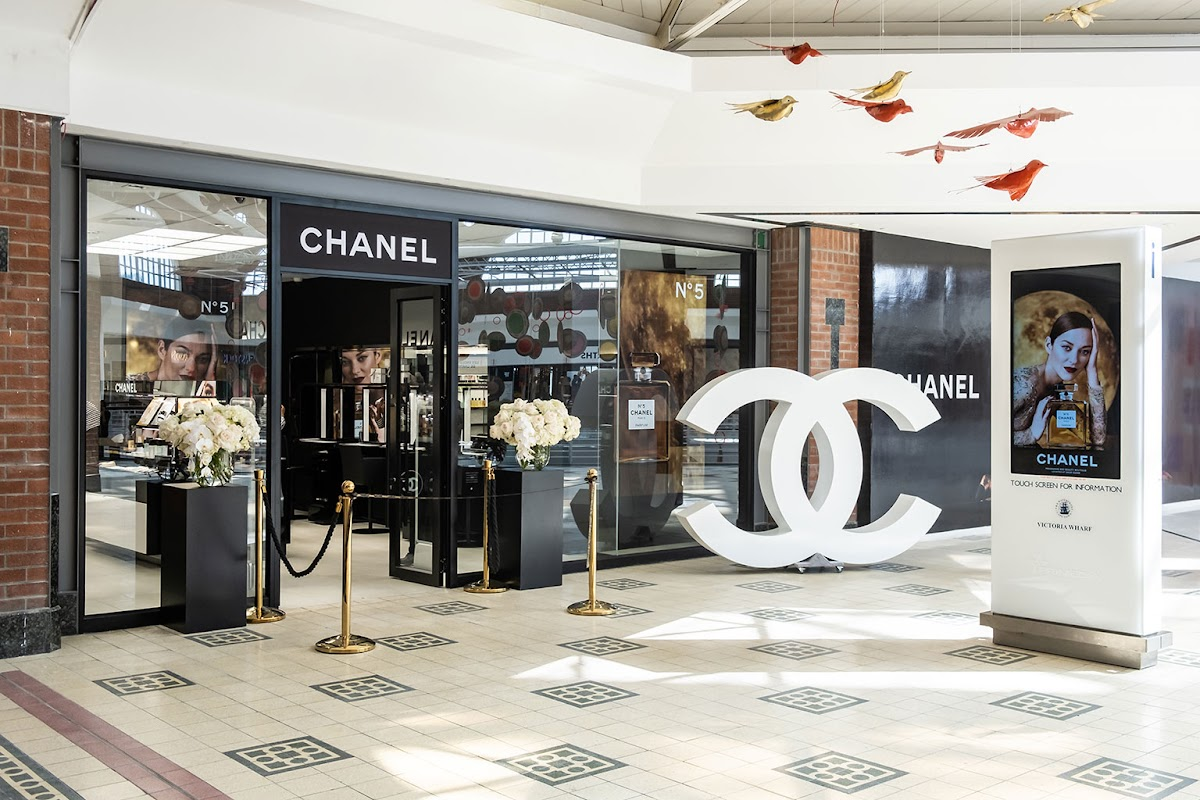
\includegraphics[width=0.49\textwidth]{chanel.png}
	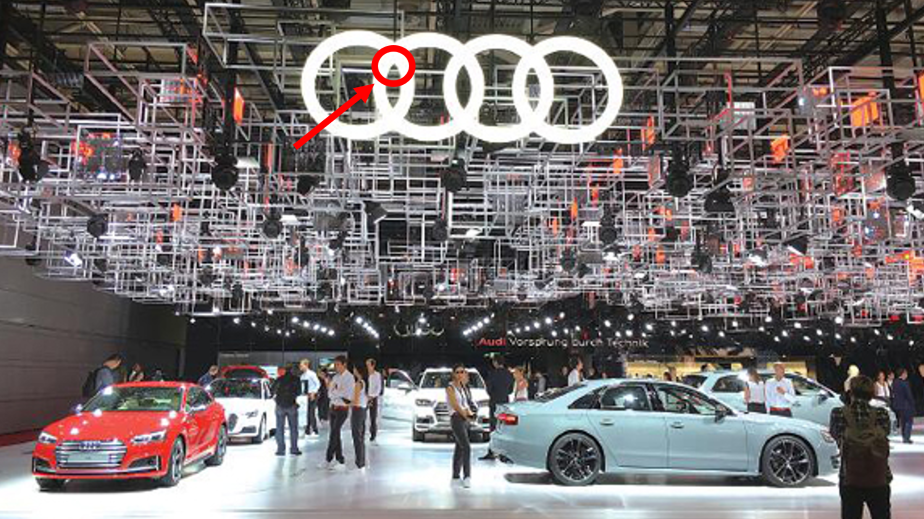
\includegraphics[width=0.49\textwidth]{audi.png}
	\caption{POI yang memiliki logo dengan sudut yang mirip.}
	\label{fig:logo_tidak_unik}
\end{figure}

Fitur lokal yang memiliki sifat konsisten dan unik tersebut dapat dicari dengan menggunakan teknik \textit{clustering}. Fitur lokal yang didapat dari gambar-gambar yang berbeda tersebut dibagi menjadi beberapa kelompok yang disebut \textit{cluster}. Dari \textit{cluster} yang terbentuk tersebut dicari kelompok mana saja yang sifatnya konsisten dan unik terhadap sebuah POI. 

\section{Analisis Terhadap Sifat-sifat Fitur Lokal pada Gambar POI}
\label{sec:analisis_sifat}
Pada \ref{sec:analisis_logo} disebutkan bahwa untuk mendapatkan fitur lokal yang berasal dari logo dan bagian konsisten serta unik perlu dicari fitur lokal yang sifatnya konsisten dan unik terhadap suatu POI tersebut. Pencarian fitur lokal konsisten dan unik tersebut dapat dilakukan dengan menggunakan teknik \textit{clustering}. 

Pada bagian ini akan dilakukan analisis untuk menguji apakah penggunaan \textit{clustering} dapat menemukan fitur lokal yang sifatnya konsisten dan unik. Dari fitur lokal yang didapatkan dari hasil \textit{clustering} tersebut ingin diperiksa apakah benar berasal dari bagian POI yang merupakan logo atau bagian lain POI yang sifatnya permanen. Bagian yang tidak permanen adalah objek-objek seperti orang-orang yang lewat.

\subsection{Ide Dasar Analisis}
\label{subsec:ide_analisis_clustering}
Analisis akan dilakukan dengan menggunakan beberapa gambar yang berbeda. Setiap gambar memiliki kelas yang merupakan POI asal gambar tersebut. Gambar dengan kelas yang sama merupakan gambar dari POI yang sama dengan sudut dan waktu pengambilan yang berbeda. Gambar-gambar tersebut diekstrak fitur lokalnya dan setiap fitur lokal ditandai asal gambarnya dan kelas dari gambar asalnya. 

Fitur-fitur lokal dari gambar tersebut lalu dibagi menjadi kelompok-kelompok dengan menggunakan teknik \textit{clustering}. Ada masalah jika ada pola tertentu pada POI yang berulang, pola berulang tersebut akan menghasilkan banyak fitur lokal dengan ciri-ciri yang mirip. Untuk mengatasi itu masing-masing gambar terlebih dahulu dilakukan \textit{clustering} pada fitur lokalnya dan dihitung \textit{centroid} untuk tiap \textit{clsuter}-nya. \textit{Centroid-centroid} ini yang nantinya akan dilakukan \textit{clustering} dengan fitur lokal dari gambar lain untuk dihitung konsistensi dan keunikannya.

Fitur lokal yang konsisten adalah fitur lokal yang muncul di semua gambar dari sebuah kelas. Kekonsistenan ini dihitung dengan melihat fitur-fitur lokal dalam sebuah \textit{cluster} jika dalam \textit{cluster} tersebut terdapat fitur lokal dari kelas A dan terdapat beberapa fitur lokal lain dari kelas yang sama tetapi dari gambar yang berbeda maka fitur lokal dengan kelas A di \textit{cluster} tersebut merupakan fitur lokal yang konsisten. Kekonsistenan ini akan ditunjukkan oleh sebuah nilai yang didapat dari menghitung jumlah gambar yang berbeda dari kelas POI yang sama dalam sebuah \textit{cluster} dan membaginya dengan jumlah gambar POI tersebut dalam dataset.

Fitur lokal unik adalah fitur lokal yang hanya muncul di satu kelas POI dan tidak muncul di POI lain. Dapat dihitung dengan fitur-fitur lokal dalam sebuah \textit{cluster}. Jika sebagian besar fitur lokal berasal dari kelas gambar A maka fitur lokal dengan kelas gambar A di \textit{cluster} tersebut merupakan fitur lokal yang unik.  Nilai keunikan didapat dari terlebih dahulu menghapus fitur lokal yang gambarnya memiliki duplikat dan lalu untuk tiap kelas gambar dihitung jumlahnya dan dibagi dengan jumlah anggota \textit{clsuter} tersebut (setelah dihapus yang duplikat).

\subsection{Tahapan Analisis}
\label{subsec:tahapan_analisis_clustering}
Langkah-langkah analisis yang dilakukan untuk mencari fitur lokal dengan sifat konsisten dan unik dapat dilihat pada \textit{flowchart} di Gambar~\ref{fig:tahapan_analisis_clustering}
\begin{figure}[H]
	\centering
	\includegraphics[scale=0.5]{tahapan\_analisis\_clustering.png}
	\caption{\textit{Flowchart} tahapan analisis \textit{clustering} untuk mencari fitur lokal yang konsisten dan unik.}
	\label{fig:tahapan_analisis_clustering}
\end{figure}

Langkah-langkah pada \textit{flowchart} di Gambar~\ref{fig:tahapan_analisis_clustering} secara rinci adalah sebagai berikut:
\begin{enumerate}
	\item \textit{Load} Gambar \\
	Pada analisis ini digunakan sebanyak total 12 gambar yang terbagi menjadi 3 kelas POI. Setiap kelas POI memiliki 4 gambar yang merupakan gambar POI tersebut dengan sudut pengambilan dan waktu pengambilan yang berbeda. Beberapa contoh gambar yang digunakan dapat dilihat pada Gambar~\ref{fig:gambar_analisis_clustering}.
	\begin{figure}[H]
		\centering
		\includegraphics[width=0.4\linewidth, height=4cm]{asus\_1\_bw2.jpg}
		\includegraphics[width=0.4\linewidth, height=4cm]{asus\_3\_bw2.jpg}
		\includegraphics[width=0.4\linewidth, height=4cm]{cgv\_1\_bw.jpg}
		\includegraphics[width=0.4\linewidth, height=4cm]{cgv\_3\_bw.jpg}
		\includegraphics[width=0.4\linewidth, height=4cm]{hnm\_1\_bw.jpg}
		\includegraphics[width=0.4\linewidth, height=4cm]{hnm\_2\_bw.jpg}
		\caption{Contoh beberapa gambar yang digunakan pada analisis ini.}
		\label{fig:gambar_analisis_clustering}
	\end{figure}
	\item Ekstraksi Fitur Lokal \\
	Lakukan ekstraksi fitur lokal dari semua gambar yang digunakan. Fitur lokal yang diekstraksi dikelompokkan berdasarkan gambar asalnya.
	\item \textit{Clustering} per Gambar \\
	Setiap kelompok fitur lokal yang telah didapat dari tahap sebelumnya digunakan untuk melakukan \textit{clustering}. Setelah didapat \textit{cluster-cluster} lalu dihitung \textit{centroid} untuk setiap \textit{cluster}. \textit{Centroid} yang telah didapat ini lalu dimasukkan kedalam satu kelompok yang sama untuk semua gambar.
	\item \textit{Clustering} pada \textit{Centroid} \\
	Setelah didapat \textit{centroid-centroid} dari hasil \textit{clustering} tiap gambar, dilakukan \textit{clustering} pada \textit{centroid-centroid} tersebut. Dari \textit{cluster-cluster} yang terbentuk dianalisis pada tahapan berikutnya.
	\item Hitung Konsistensi dan Keunikan \\
	Untuk setiap \textit{cluster} dari hasil \textit{clustering} pada \textit{centroid} dihitung nilai konsistensi dan keunikannya dengan menggunakan ide yang telah dijelaskan pada \ref{subsec:ide_analisis_clustering}. Konsistensi dan keunikan akan ditunjukkan dengan sebuah angka pada setiap \textit{centroid} dalam \textit{cluster}.
	\item Pasangkan Nilai Konsistensi dan Keunikan \\
	Pada langkah sebelumnya didapatkan nilai konsistensi dan keunikan untuk setiap \textit{centroid} hasil \textit{clustering} fitur lokal per gambar. Nilai konsistensi dan keunikan ini lalu dipasangkan ke fitur lokal asalnya sesuai dengan nomor \textit{cluster} dari \textit{clustering} tahap pertama.
	\item Analisa Fitur Lokal yang Konsisten dan Unik \\
	Setelah didapatkan nilai konsistensi dan keunikan untuk tiap fitur lokal maka akan dilakukan analisis dengan cara melakukan visualisasi fitur lokal yang memiliki nilai konsistensi dan keunikan yang tinggi untuk melihat asal fitur lokal tersebut.
\end{enumerate}

\subsection{Implementasi}
\label{subsec:tahapan_implementasi_analisis_clustering}
Langkah-langkah yang telah dijelaskan pada \ref{subsec:tahapan_analisis_clustering} dijalankan dengan membuat implementasi menggunakan Python. Versi Python yang digunakan adalah Python versi 3.7.5 dari distribusi Anaconda. Pemrosesan gambar serta ekstraksi fitur lokal dilakukan dengan menggunakan \textit{library} OpenCV versi 4.5.5.64. Untuk \textit{clustering} digunakan metode \textit{Agglomerative Clustering} dari \textit{library} Scikit-learn versi 1.0.2. Serta digunakan juga \textit{library} Pandas versi 1.3.5 untuk pemrosesan data. Langkah-langkah implementasi yang dilakukan adalah sebagai berikut:
\begin{enumerate}
	\item \textit{Import library} OpenCV (\texttt{cv2}), Scikit-learn (\texttt{sklearn}), dan Pandas (\texttt{pandas}).
	\item \textit{Load} semua gambar yang digunakan dengan fungsi \texttt{cv2.imread}. \textit{Array} gambar disimpan dalam sebuah \textit{dictionary} dengan nama gambar sebagai \textit{key}.
	\item Membuat objek SIFT dengan fungsi \texttt{cv2.SIFT\_create} masukkan ke dalam objek dengan nama \texttt{sift}.
	\item Menggunakan objek \texttt{sift} untuk melakukan ekstraksi fitur lokal dari masing-masing gambar. Ekstraksi dilakukan dengan fungsi \texttt{sift.detectAndCompute}. \textit{Keypoint} yang dihasilkan dimasukkan ke dalam sebuah \textit{list} bernama \texttt{keypoints} untuk semua gambar. Untuk deskriptor dimasukkan ke dalam sebuah \textit{dataframe} dengan nama \texttt{descriptors}.
	\item Pada \textit{dataframe} \texttt{descriptor} ditambahkan kolom \texttt{img} yang menyimpan nama gambar asal, \texttt{img\_class} untuk kelas dari gambar asal, dan \texttt{kp\_idx} yang menunjukkan posisi \textit{keypoint} di \textit{list} \texttt{keypoints}.
	\item Mengelompokkan \textit{dataframe} \texttt{descriptors} berdasarkan kolom \texttt{img} dengan menggunakan fungsi \texttt{groupby}.
	\item Melakukan iterasi untuk setiap \textit{group}. Dalam setiap iterasi lakukan \textit{clustering} pada deskriptor dengan mengambil 128 kolom pertama dari \textit{dataframe} \texttt{descriptors}. \textit{Clustering} menggunakan objek \texttt{AgglomerativeClustering} dari \texttt{sklearn} dengan parameter \texttt{distance\_threshold} didapat dari menghitung jarak rata-rata dari sampel data sebanyak 50 baris dan dibagi dua. Setelah didapat label untuk tiap \textit{cluster} dilakukan iterasi untuk tiap \textit{cluster}, pada tiap iterasi hitung \textit{centroid} dari \textit{cluster} tersebut. Hasil \textit{centroid} lalu dimasukkan ke dalam \textit{dataframe} bernama \texttt{df\_centroid}, simpan juga nomor \textit{cluster} (\texttt{cluster\_label}), nama gambar (\texttt{img}), dan kelas gambar (\texttt{img\_class}).
	\item Melakukan \textit{clustering} pada \textit{dataframe} \texttt{df\_centroid}. \textit{Clustering} juga dilakukan dengan menggunakan objek \texttt{AgglomerativeClustering} dari \texttt{sklearn}. Untuk parameter \texttt{distance\_threshold} digunakan setengah dari jarak rata-rata sampel data sebanyak 100 baris.
	Masukkan nomor \textit{cluster} sebagai kolom dengan nama \texttt{cluster2\_label} di \texttt{df\_centroid}.
	\item Membuat sebuah \textit{dictionary} bernama \texttt{cluster2\_class\_count} yang nantinya digunakan untuk menyimpan nilai keunikan.
	\item Mengelompokkan data pada \texttt{df\_centroid} berdasarkan kolom \texttt{cluster2\_label}. Untuk setiap kelompok pertama hanya ambil satu \textit{centroid} dari tiap gambar (lakukan \texttt{drop\_duplicates(subset=`img')}). Setelah itu hitung persentase banyaknya tiap kelas gambar dengan fungsi \texttt{value\_counts(normalize=True)} pada kolom \texttt{img\_class}. Masukkan hasilnya ke dalam \texttt{cluster2\_class\_count}. \textit{Dictionary} \texttt{cluster2\_class\_count} akan memiliki nomor dari \texttt{cluster2\_label} sebagai \textit{key} dan \textit{value}-nya akan berisi sebuah \textit{series} dengan \textit{key} merupakan kelas gambar dan isinya persentase kemunculan kelas gambar tersebut (nilai keunikan).
	\item Membuat sebuah \textit{list} dengan nama \texttt{uniqueness}. Isi \textit{list} tersebut dengan melakukan iterasi pada kolom \texttt{cluster2\_label} dan \texttt{img\_class} dan ambil nilai persentase keunikan yang bersesuaian dari \texttt{cluster2\_class\_count}.
	\item Memasukkan \textit{list} \texttt{uniqueness} sebagai kolom pada \texttt{df\_centroid}.
	\item Mengelompokkan \texttt{df\_centroid} berdasarkan \texttt{cluster2\_label} dan \texttt{img\_class} dengan menggunakan fungsi \texttt{groupby}. Untuk setiap kelompok dihitung jumlah gambar yang berbeda. Hasil pengelompokan dimasukkan ke dalam variabel bernama \texttt{cluster2\_img\_class\_group}.
	\item Membuat sebuah \textit{list} dengan nama \texttt{img\_count}. \textit{List} ini akan berisi nilai konsistensi untuk tiap \textit{centroid} di \texttt{df\_centroid}.
	\item Melakukan iterasi pada kolom \texttt{cluster2\_label} dan \texttt{img\_class} dari \texttt{df\_centroid}. Untuk setiap iterasi ambil nilai yang bersesuaian dari \texttt{cluster2\_img\_class\_group}. Nilai tersebut dibagi dengan 4 (jumlah gambar tiap kelas) dan dimasukkan ke dalam \textit{list} \texttt{img\_count}.
	\item Masukkan \texttt{img\_count} ke sebagai kolom di \texttt{df\_centroid} dengan nama \texttt{consistency}.
	\item Mengambil kolom \texttt{cluster\_label}, \texttt{cluster2\_label}, \texttt{uniqueness}, dan \texttt{consistency} dari \texttt{df\_centroid}. Lakukan \texttt{merge} pada kolom-kolom tersebut dengan \textit{dataframe} \texttt{descriptors} dengan bertumpu pada kolom \texttt{cluster\_label}.
	\item Mengambil \textit{keypoint} dengan nilai \texttt{consistency} dan \texttt{uniqueness} yang tinggi dan memvisualisasikan \textit{keypoint} tersebut pada gambar aslinya.
\end{enumerate}

\subsection{Hasil Analisis}
Setelah dilakukan implementasi sesuai dengan tahapan pada \ref{subsec:tahapan_implementasi_analisis_clustering} didapatkan tabel berisi deskriptor untuk \textit{keypoint} beserta dengan nilai keunikan (\texttt{uniqueness}) dan konsistensinya (\texttt{consistency}). Beberapa contoh potongan dari tabel hasil dapat dilihat pada Tabel~\ref{tab:descriptors_table}
\begin{table}[H]
	\centering
	\begin{tabular}{|c|c|c|c|c|}
		\hline
		\textbf{\texttt{img}}         & \textbf{\texttt{img\_class}} & \textbf{\texttt{cluster2\_label}} & \textbf{\texttt{uniqueness}} & \textbf{\texttt{consistency}} \\ \hline
		hnm\_1.jpg  & hnm        & 0               & 0.5        & 0.25        \\ \hline
		hnm\_1.jpg  & hnm        & 0               & 0.5        & 0.25        \\ \hline
		asus\_3.jpg & asus       & 0               & 0.5        & 0.25        \\ \hline
		hnm\_4.jpg  & hnm        & 1               & 0.5        & 0.25        \\ \hline
		cgv\_2.jpg  & cgv        & 1               & 0.5        & 0.25        \\ \hline
		cgv\_2.jpg  & cgv        & 1               & 0.5        & 0.25        \\ \hline
		cgv\_2.jpg  & cgv        & 2               & 0.66       & 0.5         \\ \hline
		hnm\_2.jpg  & hnm        & 2               & 0.33       & 0.25        \\ \hline
		cgv\_4.jpg  & cgv        & 2               & 0.66       & 0.5         \\ \hline
		cgv\_4.jpg  & cgv        & 2               & 0.66       & 0.5         \\ \hline
		cgv\_2.jpg  & cgv        & 2               & 0.66       & 0.5         \\ \hline
		cgv\_4.jpg  & cgv        & 3               & 0.5        & 0.25        \\ \hline
		asus\_4.jpg & asus       & 3               & 0.5        & 0.25        \\ \hline
		hnm\_2.jpg  & hnm        & 4               & 1          & 0.5         \\ \hline
		hnm\_3.jpg  & hnm        & 4               & 1          & 0.5         \\ \hline
		hnm\_2.jpg  & hnm        & 4               & 1          & 0.5         \\ \hline
		hnm\_2.jpg  & hnm        & 4               & 1          & 0.5         \\ \hline
		asus\_3.jpg & asus       & 5               & 0.5        & 0.25        \\ \hline
		hnm\_2.jpg  & hnm        & 5               & 0.5        & 0.25        \\ \hline
		asus\_3.jpg & asus       & 5               & 0.5        & 0.25        \\ \hline
	\end{tabular}
	\caption{Potongan beberapa contoh dari tabel deskriptor.}
	\label{tab:descriptors_table}
\end{table}

Nilai-nilai pada kolom \texttt{uniqueness} dan \texttt{consistency} didapat dari melakukan penghitungan sebaran anggota tiap \textit{cluster} seperti yang telah dijelaskan di subbab-subbab sebelumnya. Contohnya seperti semua \textit{keypoint} pada \texttt{cluster2\_label} 4 memiliki nilai keunikan yang sempurna (1) karena semua \textit{keypoint} pada \textit{cluster} tersebut berasal dari kelas (\texttt{img\_class}) yang sama. Sedangkan nilai konsistensinya hanya 0.5 karena \textit{keypoint-keypoint} dalam \textit{cluster} tersebut walaupun semua berasal dari satu kelas tetapi hanya dari 2 gambar yang berbeda, di mana seharusnya dalam satu kelas terdapat 4 gambar berbeda.

Data pada Tabel~\ref{tab:descriptors_table} menunjukkan \textit{keypoint} (fitur lokal) beserta nilai keunikan (\texttt{uniqueness}) dan konsistensinya (\texttt{consistency}). Dari tabel tersebut terlihat bahwa nilai keduanya cukup beragam. Sebaran untuk nilai keunikan dan konsistensi dapat dilihat pada Gambar~\ref{fig:hist_other_uniqueness} dan Gambar~\ref{fig:hist_other_consistency}.

\begin{figure}[H]
	\centering
	\includegraphics[width=\textwidth]{other\_uniqueness.png}
	\caption{Histogram sebaran nilai keunikan.}
	\label{fig:hist_other_uniqueness}
\end{figure}

\begin{figure}[H]
	\centering
	\includegraphics[width=\textwidth]{other\_consistency.png}
	\caption{Histogram sebaran nilai keunikan.}
	\label{fig:hist_other_consistency}
\end{figure}

\subsection{Visualisasi Keypoint yang Unik dan Konsisten}
Pada bagian ini akan dilakukan visualisasi \textit{keypoint} dalam gambar untuk melihat apakah \textit{keypoint} yang unik dan konsisten tersebut benar berasal dari bagian yang permanen dalam POI. Untuk itu \textit{keypoint-keypoint} tersebut akan disaring berdasarkan nilai keunikan dan konsistensinya. 

Penyaringan fitur lokal berdasarkan nilai keunikan dan konsistensi dilakukan dengan menetapkan suatu batas bawah untuk masing-masing nilai tersebut. Fitur lokal yang diambil untuk visualisasi adalah fitur lokal yang nilai keunikan dan konsistensinya di atas nilai-nilai batas tersebut. Penentuan batas dilakukan dengan melihat nilai persebaran keduanya dan menetukan nilai batas sehingga jumlah fitur lokal yang didapat optimal untuk melakukan visualisasi.

Sebaran untuk nilai keunikan dapat dilihat pada Gambar~\ref{fig:hist_other_uniqueness} dari subbab sebelumnya. Dari histogram pada Gambar~\ref{fig:hist_other_uniqueness} terlihat bahwa sebaran nilai keunikan tidak merata. Mayoritas \textit{keypoint} merupakan \textit{keypoint} yang unik karena memiliki nilai keunikan 1. Untuk itu akan digunakan nilai 0.9 sebagai batas pengambilan untuk visualisasi. \textit{Keypoint} dengan \texttt{uniqueness} di atas 0.9 dinilai unik dan akan diambil untuk visualisasi.

Sedangkan untuk nilai konsistensi sebarannya dapat dilihat pada Gambar~\ref{fig:hist_other_consistency}. Berbeda dengan nilai keunikan sebaran nilai konsistensi mayoritas berada pada nilai yang kecil yaitu pada rentang 0.2 - 0.3. Untuk mendapatkan \textit{keypoint} dengan jumlah yang optimal akan digunakan nilai 0.5 sebagai batas pengambilan. 

Dari hasil penyaringan menggunakan $\mathtt{uniqueness} > 0.9$ dan $\mathtt{consistency} > 0.7$ didapatkan sebanyak 785 \textit{keypoint} dari total yang berjumlah 36940. \textit{Keypoint} yang didapat tersebut lalu divisualisasikan dalam gambar beserta dengan \textit{keypoint-keypoint} yang sifatnya tidak unik dan konsisten (memiliki nilai keunikan dan konsistensi tinggi). Hasilnya dapat dilihat pada Gambar~\ref{fig:other_filtered_keypoints}.
\begin{figure}[H]
	\centering
	\includegraphics[width=\textwidth]{asus\_1\_kps.jpg}
	\includegraphics[width=\textwidth]{cgv\_2\_kps.jpg}
	\caption{Beberapa contoh \textit{keypoint} dengan nilai konsistensi dan keunikan tinggi. Lingkaran hijau merupakan \textit{Keypoint} yang nilai konsistensi dan keunikannya tinggi. Sedangkan lingkaran merah merupakan \textit{Keypoint} yang nilai konsistensi dan keunikannya rendah.}
	\label{fig:other_filtered_keypoints}
\end{figure}

Pada gambar pertama (gambar di atas) dari Gambar~\ref{fig:other_filtered_keypoints} terlihat bahwa \textit{keypoint-keypoint} yang didapat banyak yang berasal dari bagian logo atau objek yang permanen. Sebagian besar berasal dari logo di bagian atas, logo di tembok belakang dan logo di meja. Selain itu untuk \textit{keypoint} yang tidak berasal dari logo semua berasal dari bagian POI yang permanen seperti tembok, meja, atau poster. Tidak ada \textit{keypoint} yang berasal dari orang.

Sedangkan pada gambar kedua masih ada beberapa \textit{keypoint} yang berasal dari orang yang lewat. Tetapi sebagian besar \textit{keypoint} berasal dari bagian pilar yang berada di tengah gambar yang merupakan bagian permanen dari POI.

Dari hasil analisis ini didapat bahwa dengan metode \textit{clustering} seperti pada langkah-langkah di atas mampu memberikan \textit{keypoint} yang cukup unik dan konsisten. Metode mendapatkan \textit{keypoint} yang unik dan konsisten ini diharapkan dapat memberikan fitur yang kuat jika digunakan untuk melakukan OIR dengan BSIS.
%\begin{table}[H]
%	\centering
%	\begin{tabular}{|c|c|c|c|c|}
%		\hline
%		\textbf{\texttt{img}}         & \textbf{\texttt{img\_class}} & \textbf{\texttt{cluster2\_label}} & \textbf{\texttt{uniqueness}} & \textbf{\texttt{consistency}} \\ \hline
%		asus\_2.jpg & asus       & 0               & 0.75       & 0.75        \\ \hline
%		cgv\_2.jpg  & cgv        & 0               & 0.25       & 0.25        \\ \hline
%		asus\_2.jpg & asus       & 0               & 0.75       & 0.75        \\ \hline
%		asus\_2.jpg & asus       & 0               & 0.75       & 0.75        \\ \hline
%		asus\_2.jpg & asus       & 0               & 0.75       & 0.75        \\ \hline
%		asus\_2.jpg & asus       & 0               & 0.75       & 0.75        \\ \hline
%		cgv\_2.jpg  & cgv        & 0               & 0.25       & 0.25        \\ \hline
%		asus\_3.jpg & asus       & 0               & 0.75       & 0.75        \\ \hline
%		asus\_3.jpg & asus       & 0               & 0.75       & 0.75        \\ \hline
%		asus\_3.jpg & asus       & 0               & 0.75       & 0.75        \\ \hline
%		asus\_1.jpg & asus       & 0               & 0.75       & 0.75        \\ \hline
%		asus\_1.jpg & asus       & 0               & 0.75       & 0.75        \\ \hline
%		asus\_1.jpg & asus       & 0               & 0.75       & 0.75        \\ \hline
%		cgv\_2.jpg  & cgv        & 0               & 0.25       & 0.25        \\ \hline
%		cgv\_2.jpg  & cgv        & 0               & 0.25       & 0.25        \\ \hline
%		asus\_3.jpg & asus       & 0               & 0.75       & 0.75        \\ \hline
%		asus\_3.jpg & asus       & 0               & 0.75       & 0.75        \\ \hline
%		cgv\_2.jpg  & cgv        & 0               & 0.25       & 0.25        \\ \hline
%		asus\_3.jpg & asus       & 1               & 0.2        & 0.5         \\ \hline
%		hnm\_1.jpg  & hnm        & 1               & 0.4        & 1.0         \\ \hline
%	\end{tabular}
%	\caption{Potongan beberapa contoh dari tabel deskriptor.}
%	\label{tab:descriptors_table}
%\end{table}
%
%Dari Tabel~\ref{tab:descriptors_table} terlihat bahwa di \textit{cluster} dengan  \texttt{cluster2\_label} 0 terdapat 4 gambar yang berbeda. Dari 4 gambar tersebut 3 berasal dari \texttt{img\_class} \textbf{asus} dan 1 berasal dari \texttt{img\_class} \textbf{cgv}, maka \textit{keypoint} dengan \texttt{img\_class} \textbf{asus} pada \textit{cluster} tersebut akan memiliki nilai keunikan (\texttt{uniqueness}) yaitu $0.75$ dan untuk \textit{keypoint} dengan \texttt{img\_class} \textbf{cgv} memiliki nilai keunikan $0.25$. Pada \textit{cluster} tersebut juga untuk \texttt{img\_class} \textbf{asus} terdapat 3 gambar yang berbeda dari total 4 gambar yang digunakan maka nilai konsistensi (\texttt{consistency}) untuk \textit{keypoint} dengan \texttt{img\_class} \textbf{asus} pada \textit{cluster} tersebut adalah $3 / 4 = 0.75$. Sedangkan untuk \texttt{img\_class} \textbf{cgv} hanya terdapat satu gambar maka nilai konsistensinya adalah $1 / 4 = 0.25$.
%
%%\textit{Keypoint-keypoint} untuk \texttt{img\_class} \textbf{asus} pada \textit{cluster} dengan \texttt{cluster\_label} 0 tersebut merupakan \textit{keypoint} yang sifatnya unik dan konsisten karena memiliki nilai \texttt{uniqueness} dan \texttt{consistency} yang cukup tinggi. \textit{Keypoint} yang sifatnya konsisten dan unik tersebut akan divisualisasikan dalam gambar asalnya untuk melihat bagian objek dari POI yang menjadi asalnya. Hasil gambarnya dapat dilihat pada Gambar~\ref{fig:asus_keypoints}.
%
%Hasil pada Tabel~\ref{tab:descriptors_table} menunjukkan bahwa ada beberapa \textit{keypoint} yang memiliki nilai keunikan dan konsistensi yang tinggi dan ada beberapa yang rendah. Dengan menggunakan data tersebut \textit{keypoint} akan disaring berdasarkan nilainya keunikan dan konsistensinya dan dilakukan visualisasi. Akan dianalisis apakah \textit{keypoint} yang unik dan konsisten berasal dari bagian yang merupakan logo atau bagian dari POI yang bukan merupakan objek latar belakang atau objek yang tidak tetap. 
%
%\begin{figure}[H]
%	\centering
%	\includegraphics[width=\textwidth]{asus\_2\_kps.jpg}
%	\includegraphics[width=\textwidth]{asus\_3\_kps.jpg}
%	\caption{Beberapa contoh \textit{keypoint} dengan nilai konsistensi dan keunikan tinggi. \textit{Keypoint} ditandai dengan lingkaran merah pada gambar.}
%	\label{fig:asus_keypoints}
%\end{figure}

%Dari kedua gambar tersebut terlihat bahwa sebagian besar \textit{keypoint} berasal dari bagian yang merupakan logo. Terutama di gambar kedua (gambar yang di bawah) semua \textit{keypoint} yang ditampilkan berasal dari logo POI baik yang berada di bagian atas POI maupun logo yang berada di bagian meja. Sedangkan untuk gambar yang pertama hanya beberapa \textit{keypoint} yang berasal dari logo sisanya berasal dari bagian lain dari POI. Walaupun begitu \textit{keypoint} yang berasal dari objek lain semuanya tidak ada yang berasal dari orang (pengunjung).
%
%Tahapan \textit{clustering} yang dilakukan ini dapat digunakan untuk menyaring \textit{fitur lokal} untuk didapatkan yang kuat saja. Pada tahapan selanjutnya akan dianalisis apakah dengan menyaring fitur lokal dan mengambil yang kuat (konsisten dan unik) saja dapat digunakan untuk melakukan OIR dengan BSIS. 

\section{Analisis Penggunaan Clustering untuk OIR dengan BSIS}
\label{sec:analisis_bsis}
Pada analisis sebelumnya telah diterapkan metode \textit{clustering} untuk mencari fitur lokal yang unik dan konsisten. Fitur lokal yang unik dan konsisten tersebut diharapkan dapat menjadi fitur yang kuat untuk melakukan identifikasi sebuah gambar. Penelitian kali ini dilakukan dengan menggunakan dataset bernama Book Covers yang berisi gambar cover buku. Dataset tersebut digunakan karena gambar-gambar yang ada dinilai cukup mirip dengan POI, di mana dalam sebuah gambar ada objek inti yang menyerupai logo dan objek latar belakang juga karena pada tahap ini belum dilakukan pengumpulan data. 

Analisis dilakukan dengan melakukan identifikasi sejumlah gambar tes terhadap dataset yang menggunakan semua fitur lokal dan dataset yang menggunakan fitur lokal yang telah disaring berdasarkan keunikan dan kekonsistenannya. Hasil tes keduanya lalu dibandingkan tingkat akurasi dan waktu pemrosesannya. Proses identifikasi dilakukan dengan menggunakan metode BSIS~\ref{sec:bsis}.

\subsection{Data Train dan Test}
\subsubsection{Data Train}
Data \textit{train} yang digunakan berjumlah total sebanyak 200 gambar yang terbagi menjadi 50 kelas. Tiap kelas berjumlah 4 gambar buku yang sama diambil dari sudut pengambilan yang berbeda dan terdapat objek di latar belakang yang berbeada. Salah satu contoh kelas dari dataset dapat dilihat pada Gambar~\ref{fig:contoh_book_covers}.
\begin{figure}[H]
	\centering
	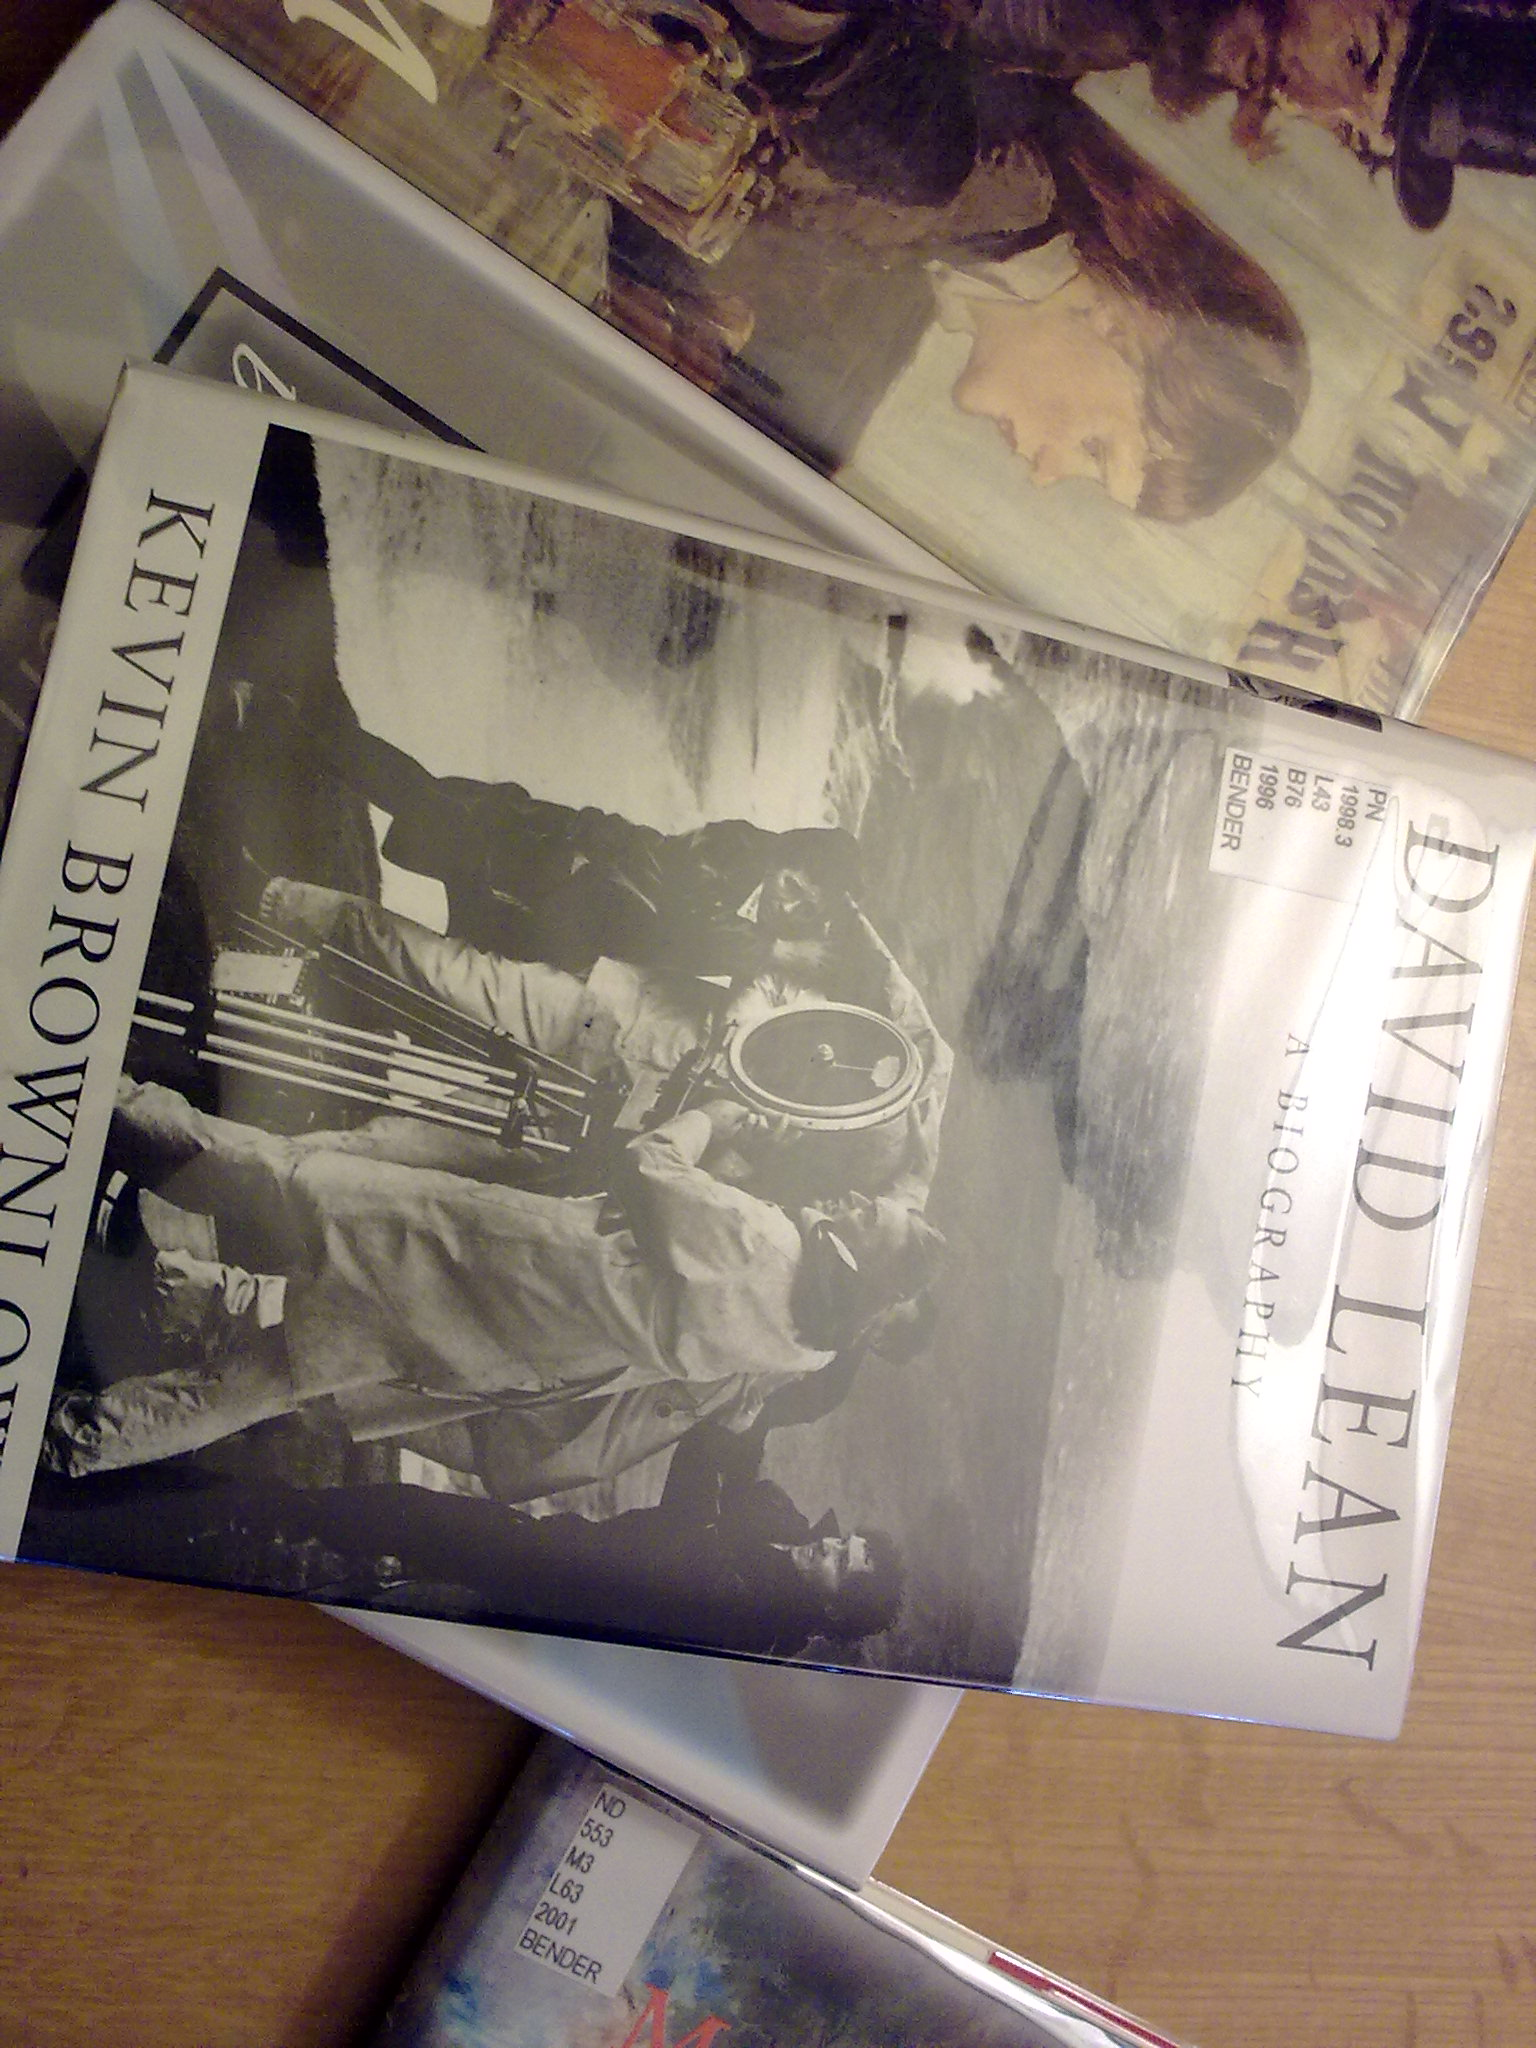
\includegraphics[width=0.24\textwidth, angle=0]{013-5800.jpg}
	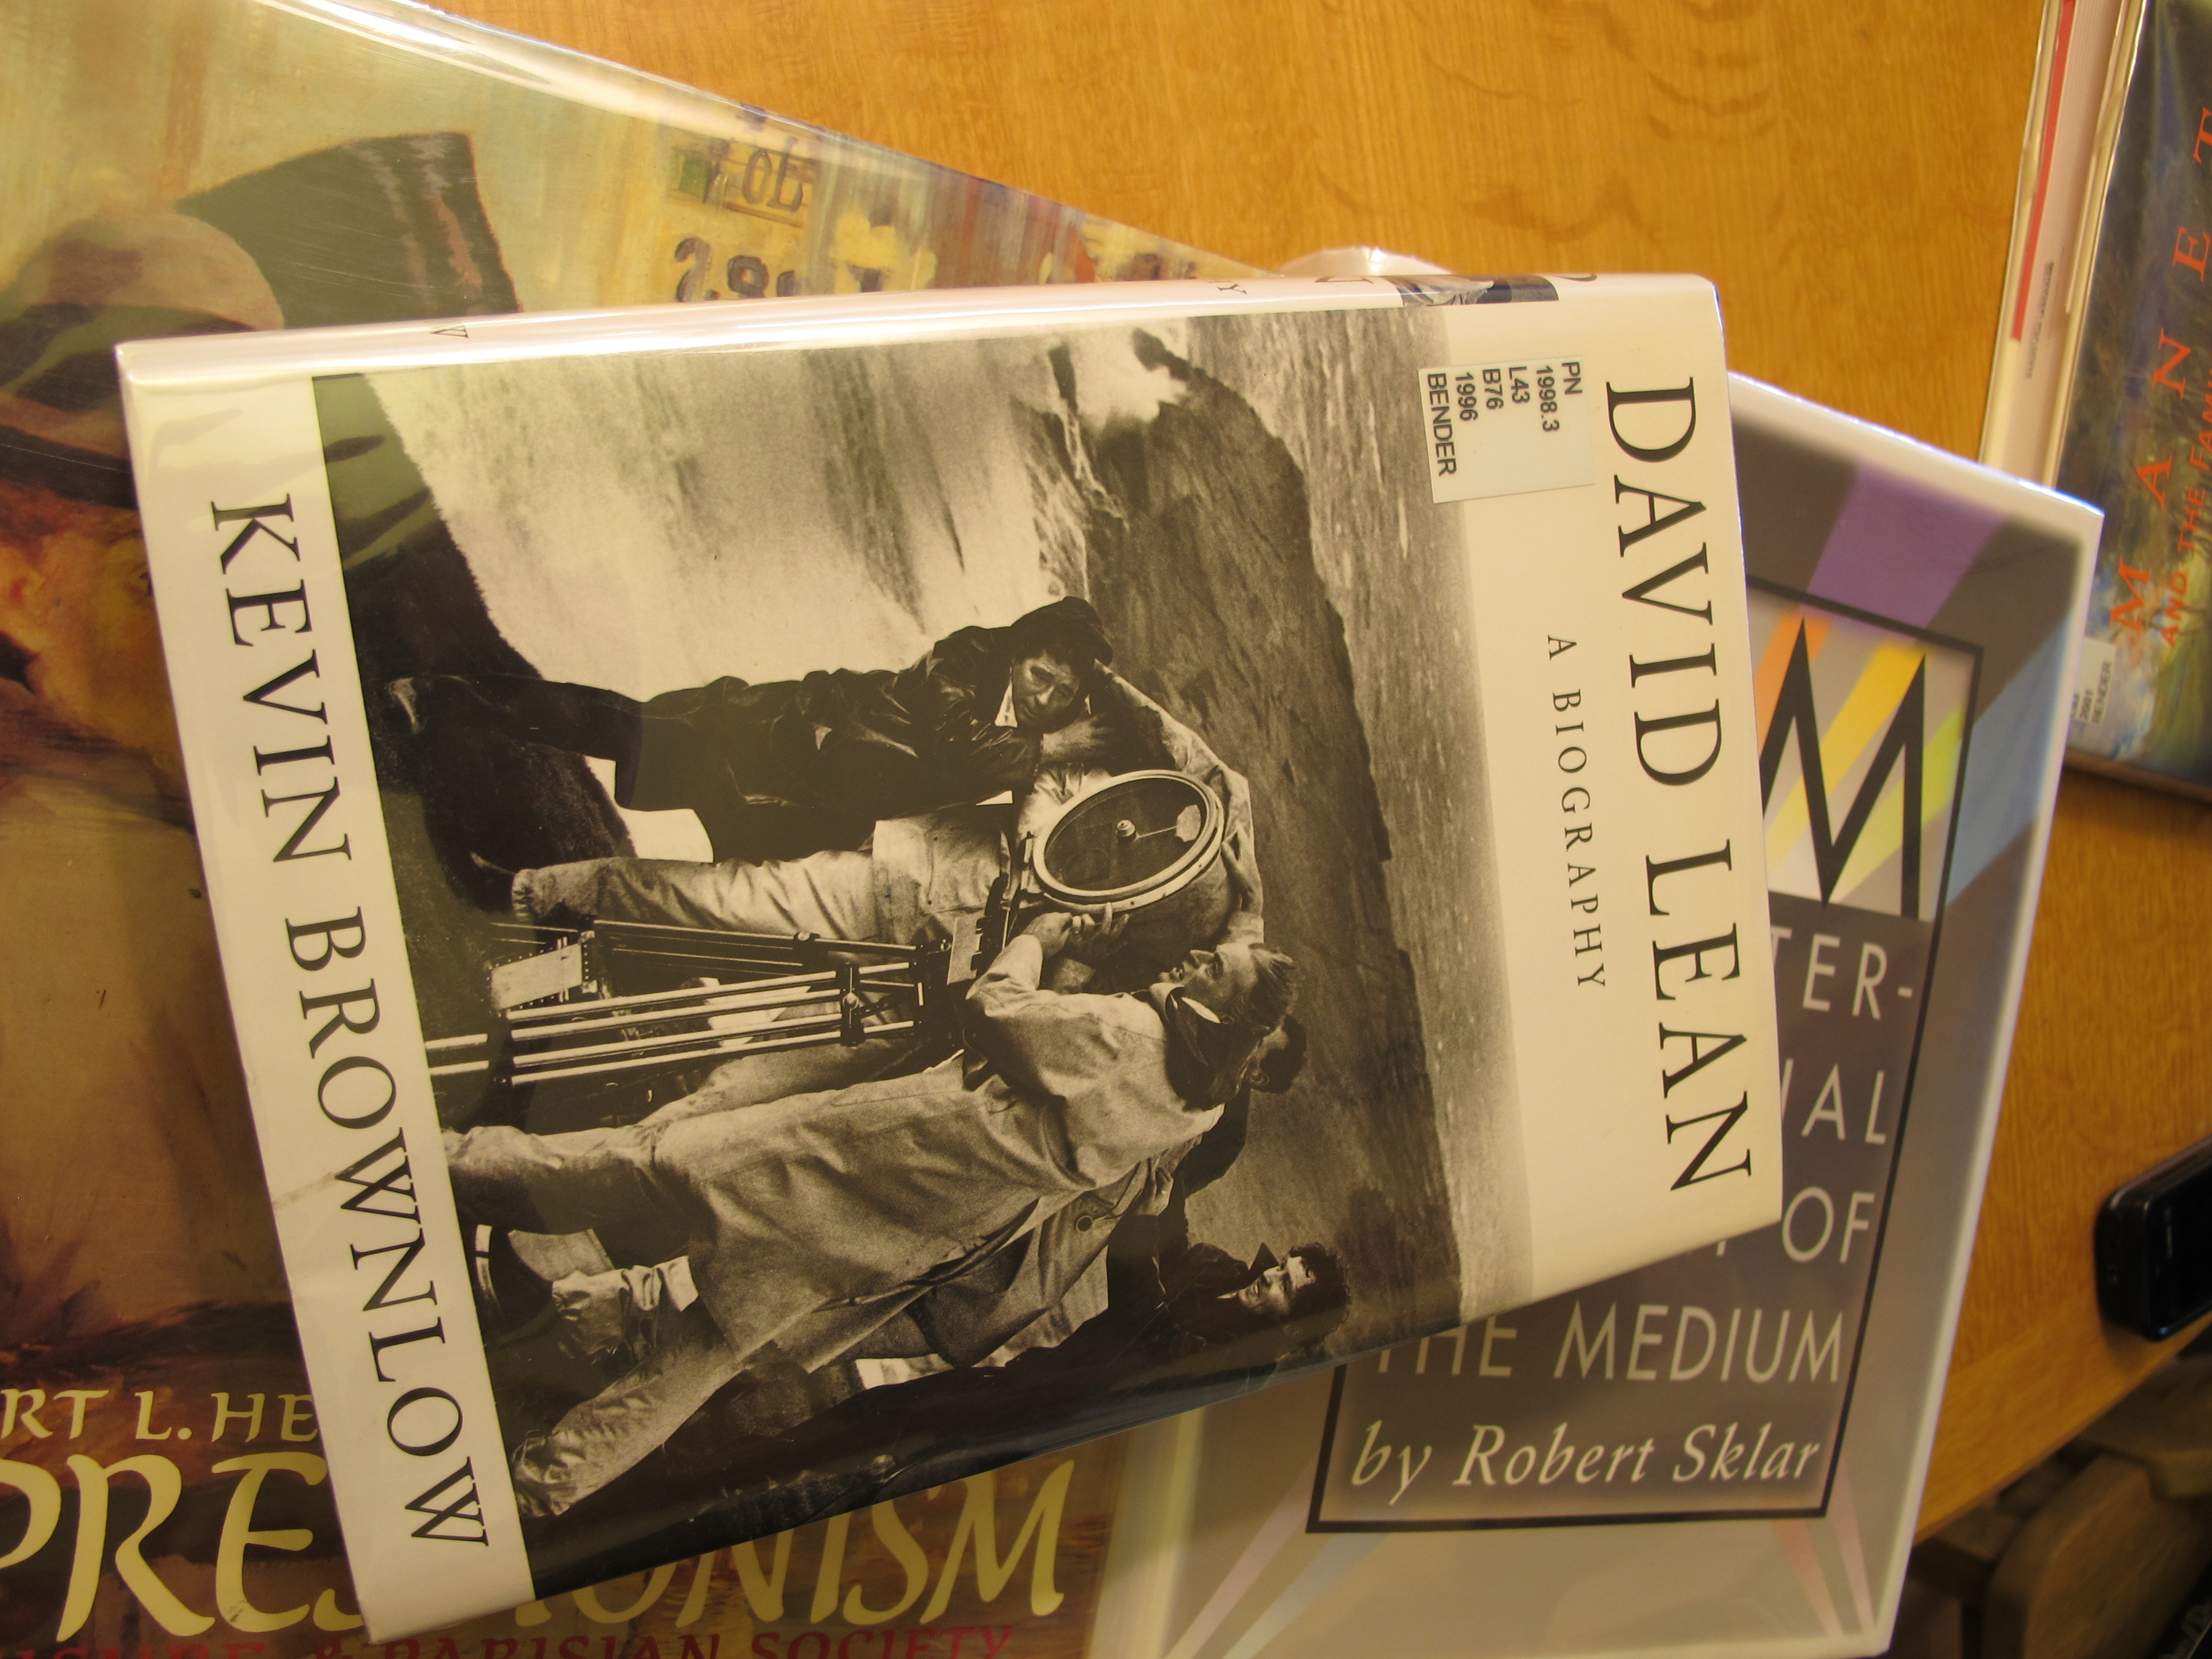
\includegraphics[width=0.24\textwidth, angle=0]{013-Canon.jpg}
	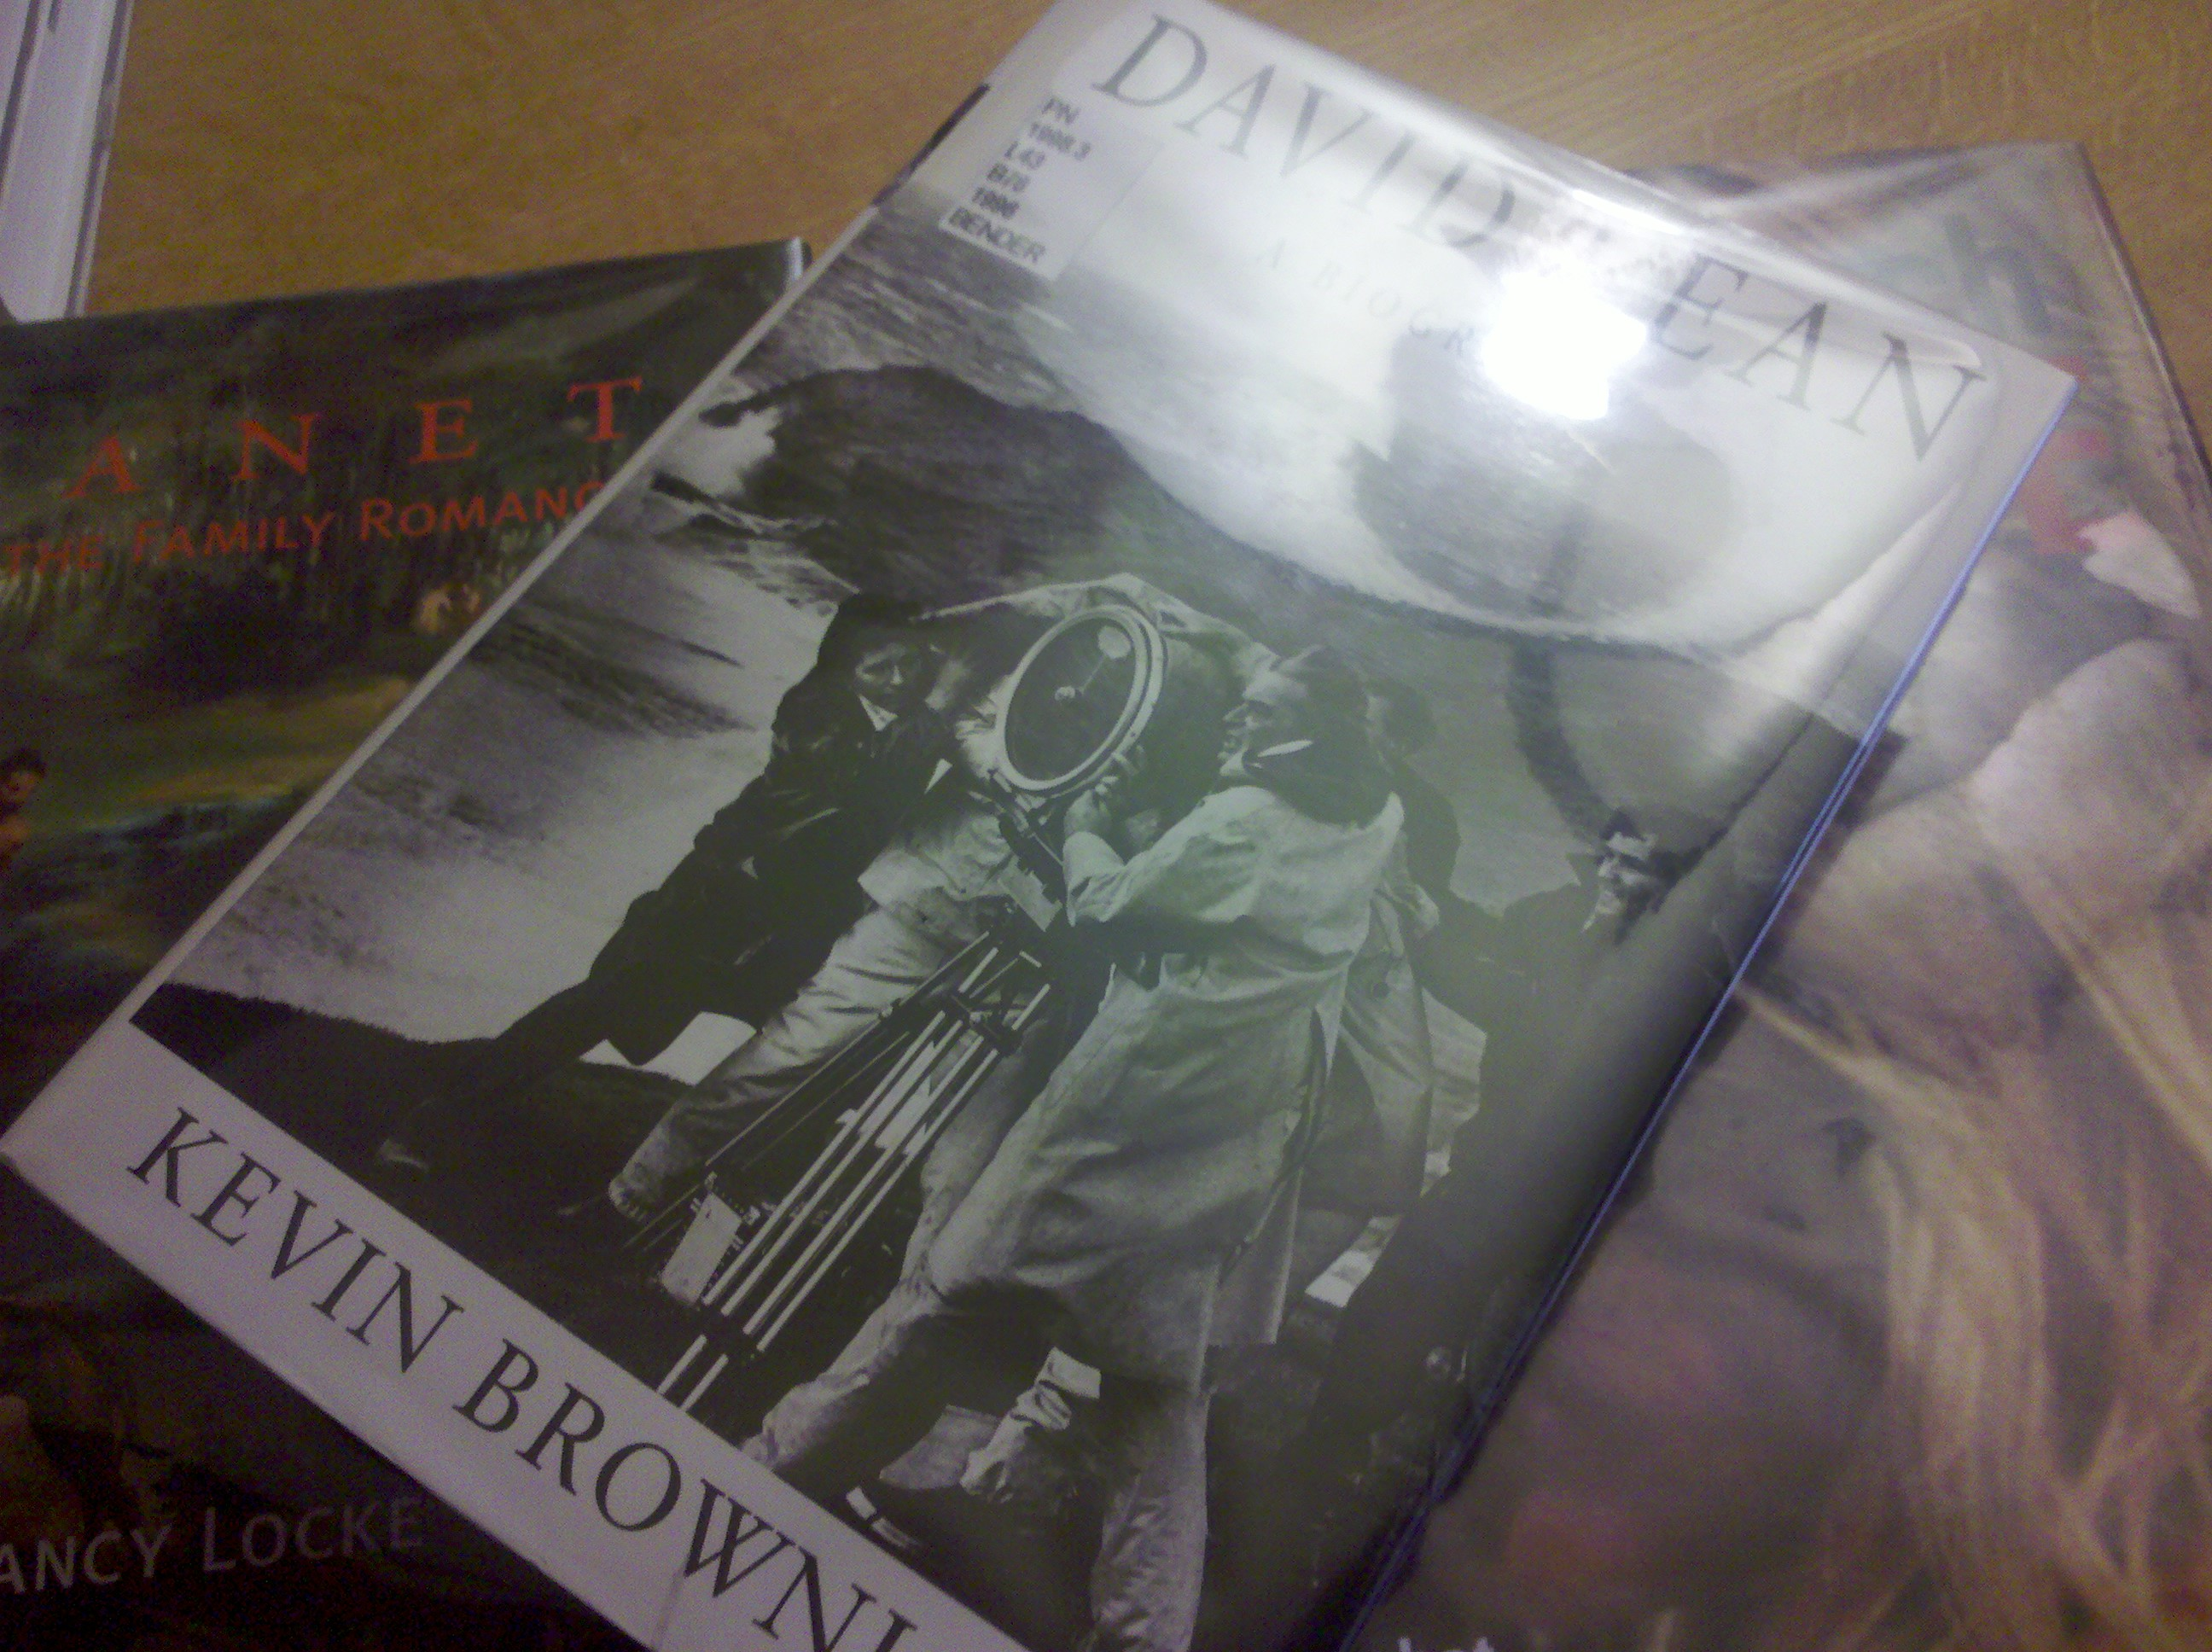
\includegraphics[width=0.24\textwidth, angle=0]{013-Droid.jpg}
	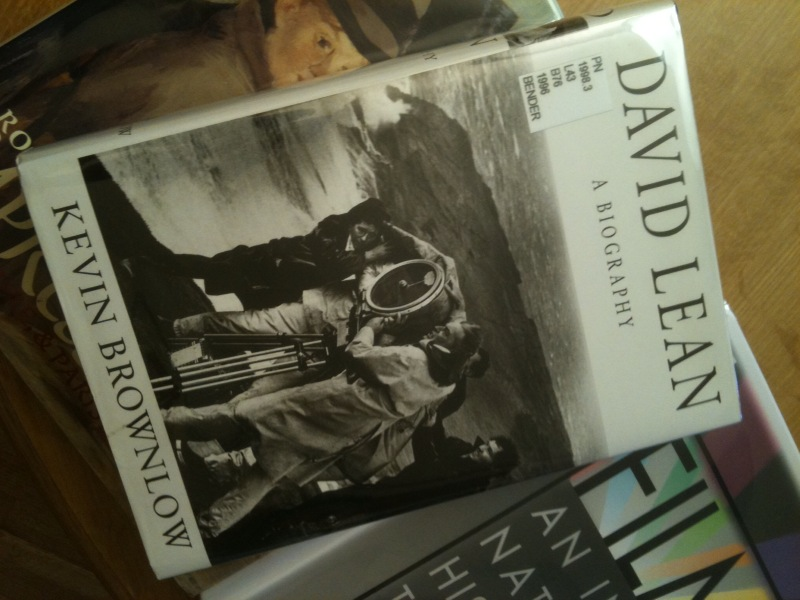
\includegraphics[width=0.24\textwidth, angle=0]{013-iPhone.jpg}
	\caption{Contoh gambar pada dataset Book Covers. Keempat gambar tersebut berada dalam satu kelas yang sama.}
	\label{fig:contoh_book_covers}
\end{figure}

Data \textit{train} yang sama digunakan dua kali dengan ukuran yang berbeda. Ukuran gambar diperkecil sehingga sisi paling panjangnya tidak lebih dari 400 \textit{pixel} untuk set pertama dan tidak lebih dari 600 \textit{pixel} untuk set kedua. Ukuran gambar yang berbeda akan menghasilkan jumlah fitur lokal yang berbeda juga, semakin besar ukurannya maka semakin banyak fitur lokal yang dihasilkan. Penggunaan ukuran yang berbeda ini bertujuan untuk melihat apakah ada perbedaan akurasi jika ukuran gambar pada dataset berubah.

Gambar-gambar tersebut diekstrak fitur lokalnya dan untuk setiap fitur lokal dihitung nilai konsistensi dan keunikan menggunakan metode seperti pada \ref{sec:analisis_sifat}. Karena keterbatasan \textit{memory} pada perangkat yang digunakan jumlah fitur lokal yang diekstrak dari tiap gambar dibatasi sebanyak 250 fitur lokal.

\subsubsection{Data Test}
Data \textit{test} yang digunakan diambil dari gambar referensi dataset Book Covers. Gambar referensi merupakan gambar buku yang menjadi objek utama dalam setiap kelas dengan kondisi yang ideal. Contoh gambar referensi dapat dilihat pada Gambar~\ref{fig:referensi_book_covers}.

\begin{figure}[H]
	\centering
	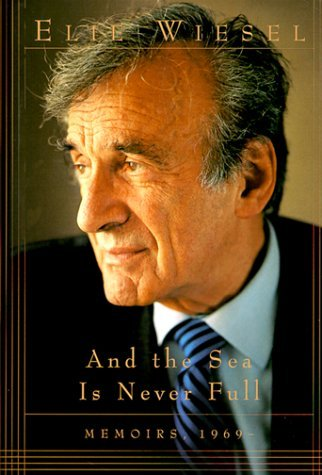
\includegraphics[width=0.3\textwidth]{004.jpg}
	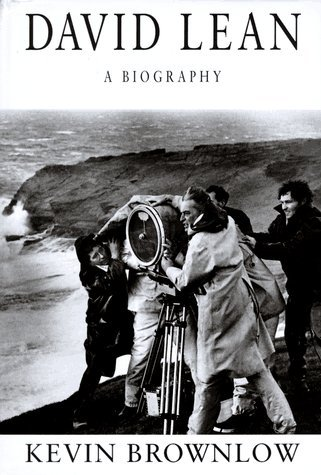
\includegraphics[width=0.3\textwidth]{013.jpg}
	\caption{Contoh gambar referensi dari dataset Book Covers.}
	\label{fig:referensi_book_covers}
\end{figure}

Gambar-gambar referensi tersebut berjumlah total 50 gambar masing-masing untuk tiap kelas. Dari 50 gambar tersebut lalu ditransformasi dengan mengubah tingkat perbesaran dan rotasi secara acak. Transformasi tersebut dilakukan sebanyak dua kali untuk tiap gambar. Contoh gambar referensi yang telah ditransformasi dapat dilihat pada Gambar~\ref{fig:transformasi_book_covers}. Masing-masing hasil transformasi disimpan sebagai satu gambar sehingga terdapat total sebanyak 100 gambar untuk data \textit{test}.

Data \textit{test} yang berjumlah 100 tersebut memiliki ukuran lebar yang berkisar antara $133 - 441$ \textit{pixel}, sedangkan untuk tingginya berkisar antara $198 - 502$ \textit{pixel}.

\begin{figure}[H]
	\centering
	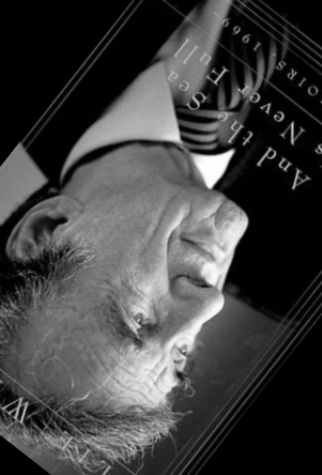
\includegraphics[width=0.3\textwidth]{004-test1.jpg}
	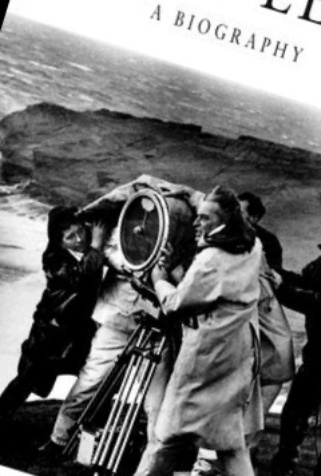
\includegraphics[width=0.3\textwidth]{013-test1.jpg}
	\caption{Contoh gambar referensi dari dataset Book Covers.}
	\label{fig:transformasi_book_covers}
\end{figure}

\subsection{Metode BSIS}
Analisis ini akan melakukan identifikasi terhadap gambar yang dilakukan menggunakan metode BSIS seperti yang telah dijelaskan pada \ref{sec:bsis}. Metode BSIS sendiri secara garis besar terdiri dari 3 langkah sebagai berikut:
\begin{enumerate}
	\item \textit{Pairing} \\
	Untuk setiap fitur lokal pada gambar \textit{test} dibuat pasangan dengan memasangkannya pada fitur lokal dari dataset \textit{train}.
	\item \textit{Verification} \\
	Dari pasangan-pasangan yang terbentuk dari tahap sebelumya dilakukan verifikasi untuk mencari pasangan yang konsisten secara geometris.
	\item \textit{Scoring} \\
	Setelah didapat pasangan-pasangan yang memilki sifat konsisten secara geometris dihitung total bobot dari pasangan-pasangan tersebut sebagai nilai yang menunjukkan kemiripan dua buah gambar tersebut.
\end{enumerate}
Pada analisis ini dilakukan sedikit modifikasi pada metode BSIS, modifikasi dilakukan seperti yang ditunjukkan pada Gambar~\ref{fig:bsis_mod}
\begin{figure}[H]
	\centering
	\includegraphics[width=\textwidth]{bsis\_mod.png}
	\caption{Modifikasi pada metode BSIS yang dilakukan pada analisis ini.}
	\label{fig:bsis_mod}
\end{figure}

Terdapat tahap \textit{clustering} yang dilakukan terhadap dataset \textit{train} sebelum melakukan \textit{pairing}, sehingga \textit{pairing} dilakukan terhadap dataset \textit{train} yang telah disaring berdasarkan hasil \textit{clustering}. Tahap penyaringan akan menyebabkan fitur lokal dataset \textit{train} yang perlu diperiksa menjadi lebih sedikit. Hal ini akan mempercepat waktu yang diperlukan untuk melakukan \textit{pairing}.


\subsection{Tahapan Analisis}
Analisis dilakukan dengan tahapan pada dua dataset yang berbeda dengan tahapan yang sama. Dataset pertama akan disebut Dataset 400 yang menggunakan gambar dengan ukuran sisi terbesarnya tidak lebih dari 400 \textit{pixel}. Dataset kedua disebut Dataset 600 yang ukuran sisi terbesarnya tidak lebih dari 600 \textit{pixel}. Tahapan analisis yang dilakukan dapat dilihat pada \textit{flowchart} di Gambar~\ref{fig:tahapan_analisis_bsis}.
\begin{figure}
	\centering
	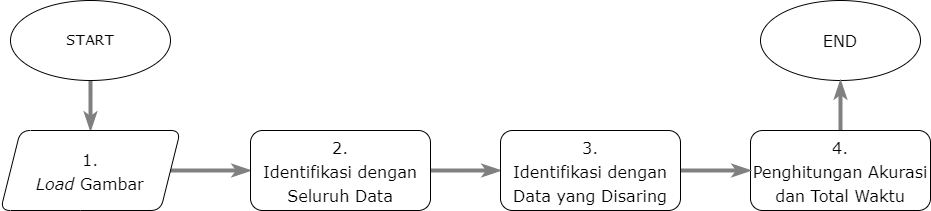
\includegraphics[width=\textwidth]{tahapan_analisis_bsis.png}
	\caption{Tahapan yang dilakukan dalam analisis untuk menguji penggunaan \textit{clustering} pada BSIS.}
	\label{fig:tahapan_analisis_bsis}
\end{figure}
Secara rinci tahapan yang dilakukan adalah sebagai berikut:
\begin{enumerate}
	\item \textit{Load} Gambar \\
	\textit{Load} semua gambar \texttt{test} yang digunakan.
	\item Identifikasi dengan BSIS pada seluruh Dataset \\
	Untuk masing-masing gambar \textit{test} lakukan ekstraksi fitur lokal dan gunakan fitur lokal tersebut untuk melakukan identifikasi BSIS dengan menggunakan seluruh fitur lokal pada dataset. Untuk setiap gambar hitung waktu yang digunakan untuk melakukan BSIS hingga didapat hasilnya. Total waktu tidak termasuk waktu yang digunakan untuk ekstraksi fitur.
	\item Identifikasi dengan BSIS pada Dataset yang Telah Disaring \\
	Lakukan kembali identifikasi seluruh gambar \textit{test} tetapi dengan menggunakan hanya sebagian dataset yang telah disaring berdasarkan nilai keunikan dan konsistensinya.
	\item Penghitungan Akurasi dan Total Waktu \\
	Hitung total waktu yang digunakan untuk menyelesaikan seluruh gambar dan berapa gambar yang mendapat hasil benar.
\end{enumerate}
Tahapan tersebut dilakukan sebanyak 2 kali untuk masing-masing Dataset 400 dan Dataset 600. Setelah didapat hasil akurasi dan total waktu untuk Dataset 400 dan Dataset 600 bandingkan keduanya dan lakukan analisis.

\subsection{Tahapan Implementasi}
Implementasi dilakukan dengan membuat program Python. Digunakan Python versi 3.7.5 dengan \textit{library} OpenCV versi 4.5.5.64 untuk pemrosesan gambar dan Pandas versi 1.3.5 untuk memroses data. Langkah-langkah implementasi yang dilakukan adalah sebagai berikut:
\begin{enumerate}
	\item \texttt{Import library} yang digunakan: OpenCV (\texttt{cv2}) dan Pandas (\texttt{pandas}).
	\item \textit{Load} gambar \textit{test} masukkan ke dalam variabel \textit{list} bernama \texttt{test\_dataset}. Setiap elemen dalam \texttt{test\_dataset} berupa \textit{tuple} dengan dua elemen. Elemen pertama merupakan nama gambar dan elemen kedua merupakan \textit{array} gambar tersebut.
	\item \textit{Load} dataset yang digunakan untuk data \textit{train}.
	\item Menentukan parameter batas nilai \texttt{uniqueness} dan \texttt{consistency} untuk menyaring dataset. 
	\item Membuat objek SIFT dengan fungsi \texttt{cv2.SIFT\_create()}.
	\item Membuat 5 buah \textit{list} untuk menyimpan hasil deteksi. Dengan rincian sebagai berikut:
	\begin{itemize}
		\item \texttt{q\_name}: Untuk menyimpan nama dari gambar \textit{test}.
		\item \texttt{t\_name}: Nama gambar yang paling mirip berdasarkan hasil BSIS.
		\item \texttt{kdtree\_time}: Waktu yang diperlukan implementasi KD-Tree untuk mencari $n$ pasangan paling mirip untuk semua fitur lokal di gambar \textit{test}.
		\item \texttt{total\_time}: Total waktu yang diperlukan oleh BSIS hingga memberikan hasil.
		\item \texttt{total\_weight}: Total bobot pasangan yang dibentuk oleh BSIS.
	\end{itemize}
	\item Mengiterasi \texttt{test\_dataset} dan masukkan nama gambar ke \texttt{q\_name}. Pada setiap iterasi terlebih dahulu melakukan ekstraksi fitur lokal dari gambar \textit{test} dengan fungsi \texttt{sift.detectAndCompute}. 
	\item Menggunakan \textit{keypoint} dan deskriptor dari fitur lokal gambar untuk melakukan BSIS.
	\item Mengisi \textit{list} \texttt{t\_name}, \texttt{kdtree\_time}, \texttt{total\_time}, dan \texttt{total\_weight} dengan hasil dari BSIS.
	\item Menggabungkan \textit{list} \texttt{q\_name}, \texttt{t\_name}, \texttt{kdtree\_time}, \texttt{total\_time}, dan \texttt{total\_weight} ke dalam sebuah \textit{dataframe}.
	\item Untuk setiap baris di \textit{dataframe} memeriksa apakah hasilnya benar. Hasil dinilai benar jika gambar \textit{train} yang didapat dari hasil BSIS (gambar pada \texttt{t\_name}) merupakan salah satu dari 4 gambar yang berada pada kelas yang sama dengan gambar \textit{test}.
	\item Melakukan lagi langkah 5-10 dengan dataset yang telah disaring berdasarkan nilai batas \texttt{uniqueness} dan \texttt{consistency} yang telah ditentukan sebelumnya.
\end{enumerate}
Langkah-langkah tersebut dilakukan untuk Dataset 400 dan Dataset 600. Hasil dari kedua dataset tersebut lalu dibandingkan.

\subsection{Hasil Implementasi}
\subsubsection{Dataset 400}
Dataset 400 memiliki total fitur lokal yang dihasilkan dari seluruh gambar sebanyak 49524 fitur lokal. Setelah dilakukan \textit{clustering} menghitung nilai keunikan dan konsistensi didapat hasil sebaran nilai keunikan dan konsistensi seperti pada Gambar~\ref{fig:half_400_uniqueness} dan Gambar~\ref{fig:half_400_consistency}.
\begin{figure}[H]
	\centering
	\includegraphics[width=\textwidth]{half\_400\_uniqueness.png}
	\caption{Sebaran nilai keunikan (\texttt{uniqueness}) untuk Dataset 400.}
	\label{fig:half_400_uniqueness}
\end{figure}
\begin{figure}[H]
	\centering
	\includegraphics[width=\textwidth]{half\_400\_consistency.png}
	\caption{Sebaran nilai keunikan (\texttt{consistency}) untuk Dataset 400.}
	\label{fig:half_400_consistency}
\end{figure}
Berdasarkan sebaran data tersebut ditentukan batas untuk nilai keunikan (\texttt{uniqueness}) adalah $> 0.99$ dan untuk konsistensi (\texttt{consistency}) adalah $> 0.49$. Setelah data disaring menggunakan batas-batas tersebut didapatkan total sebanyak 13281 fitur lokal. Data keseluruhan dan data yang telah disaring tersebut lalu digunakan untuk pengenalan gambar \textit{test}. 

Hasil pengenalan gambar \textit{test} pada dataset keseluruhan dapat dilihat potongannya pada Tabel~\ref{tab:result_full_400}.
\begin{table}[H]
	\centering
	\begin{tabular}{|c|c|c|c|c|c|c|} 
		\hline
		& \textbf{q\_name}       & \textbf{t\_name}        & \textbf{kdtree\_time} & \textbf{total\_time} & \textbf{total\_weight} & \textbf{is\_true}  \\ 
		\hline
		0   & 001-test0.jpg & 001-iPhone.jpg & 1.218        & 1.331       & 118.152       & 1         \\ 
		\hline
		1   & 001-test1.jpg & 001-Droid.jpg  & 1.142        & 1.235       & 81.080        & 1         \\ 
		\hline
		2   & 002-test0.jpg & 002-Droid.jpg  & 1.038        & 1.082       & 75.547        & 1         \\ 
		\hline
		3   & 002-test1.jpg & 002-Droid.jpg  & 1.044        & 1.094       & 59.720        & 1         \\ 
		\hline
		4   & 003-test0.jpg & 003-iPhone.jpg & 1.076        & 1.164       & 147.223       & 1         \\ 
		\hline
		5   & 003-test1.jpg & 003-iPhone.jpg & 1.079        & 1.188       & 187.710       & 1         \\ 
		\hline
		6   & 004-test0.jpg & 004-iPhone.jpg & 1.024        & 1.061       & 278.902       & 1         \\ 
		\hline
		7   & 004-test1.jpg & 004-iPhone.jpg & 1.100        & 1.218       & 500.139       & 1         \\ 
		\hline
		8   & 005-test0.jpg & 005-Droid.jpg  & 0.839        & 0.998       & 888.100       & 1         \\ 
		\hline
		9   & 005-test1.jpg & 005-Droid.jpg  & 0.747        & 0.897       & 737.421       & 1         \\ 
		\hline
		... & ...           & ...            & ...          & ...         & ...           & ...       \\ 
		\hline
		90  & 046-test0.jpg & 046-iPhone.jpg & 0.691        & 0.736       & 192.444       & 1         \\ 
		\hline
		91  & 046-test1.jpg & 046-iPhone.jpg & 0.710        & 0.770       & 220.680       & 1         \\ 
		\hline
		92  & 047-test0.jpg & 047-iPhone.jpg & 0.692        & 0.737       & 306.918       & 1         \\ 
		\hline
		93  & 047-test1.jpg & 047-iPhone.jpg & 0.674        & 0.690       & 40.375        & 1         \\ 
		\hline
		94  & 048-test0.jpg & 048-iPhone.jpg & 0.658        & 0.690       & 409.121       & 1         \\ 
		\hline
		95  & 048-test1.jpg & 048-iPhone.jpg & 0.661        & 0.683       & 288.478       & 1         \\ 
		\hline
		96  & 049-test0.jpg & 049-iPhone.jpg & 0.717        & 0.825       & 465.788       & 1         \\ 
		\hline
		97  & 049-test1.jpg & 049-iPhone.jpg & 0.698        & 0.789       & 413.234       & 1         \\ 
		\hline
		98  & 050-test0.jpg & 050-Canon.jpg  & 0.872        & 1.047       & 77.518        & 1         \\ 
		\hline
		99  & 050-test1.jpg & 044-Droid.jpg  & 0.796        & 0.930       & 33.449        & 0         \\
		\hline
	\end{tabular}
	\caption{Beberapa contoh hasil BSIS pada keseluruhan Dataset 400.}
	\label{tab:result_full_400}
\end{table}

Sedangkan untuk hasil pada data yang telah disaring beberapa potongannya adalah seperti dapat dilihat pada Tabel~\ref{tab:result_filtered_400}
\begin{table}[H]
	\centering
	\begin{tabular}{|c|c|c|c|c|c|c|} 
		\hline
		& \textbf{q\_name} & \textbf{t\_name} & \textbf{kdtree\_time} & \textbf{total\_time} & \textbf{total\_weight} & \textbf{is\_true}  \\ 
		\hline
		0   & 001-test0.jpg    & 001-iPhone.jpg   & 0.395                 & 0.510                & 74.987                 & 1                  \\ 
		\hline
		1   & 001-test1.jpg    & 001-Droid.jpg    & 0.368                 & 0.465                & 58.541                 & 1                  \\ 
		\hline
		2   & 002-test0.jpg    & 002-iPhone.jpg   & 0.313                 & 0.353                & 53.240                 & 1                  \\ 
		\hline
		3   & 002-test1.jpg    & 002-Droid.jpg    & 0.321                 & 0.360                & 56.742                 & 1                  \\ 
		\hline
		4   & 003-test0.jpg    & 003-Droid.jpg    & 0.357                 & 0.450                & 112.820                & 1                  \\ 
		\hline
		5   & 003-test1.jpg    & 003-Droid.jpg    & 0.337                 & 0.440                & 147.134                & 1                  \\ 
		\hline
		6   & 004-test0.jpg    & 004-iPhone.jpg   & 0.283                 & 0.308                & 58.114                 & 1                  \\ 
		\hline
		7   & 004-test1.jpg    & 004-iPhone.jpg   & 0.365                 & 0.478                & 59.555                 & 1                  \\ 
		\hline
		8   & 005-test0.jpg    & 005-Droid.jpg    & 0.372                 & 0.548                & 326.424                & 1                  \\ 
		\hline
		9   & 005-test1.jpg    & 005-Droid.jpg    & 0.375                 & 0.574                & 364.295                & 1                  \\ 
		\hline
		... & ...              & ...              & ...                   & ...                  & ...                    & ...                \\ 
		\hline
		90  & 046-test0.jpg    & 046-iPhone.jpg   & 0.200                 & 0.245                & 150.351                & 1                  \\ 
		\hline
		91  & 046-test1.jpg    & 046-iPhone.jpg   & 0.211                 & 0.272                & 229.700                & 1                  \\ 
		\hline
		92  & 047-test0.jpg    & 047-iPhone.jpg   & 0.202                 & 0.248                & 133.144                & 1                  \\ 
		\hline
		93  & 047-test1.jpg    & NaN              & 0.190                 & 0.204                & 0.000                  & 0                  \\ 
		\hline
		94  & 048-test0.jpg    & 048-iPhone.jpg   & 0.174                 & 0.197                & 243.964                & 1                  \\ 
		\hline
		95  & 048-test1.jpg    & 048-iPhone.jpg   & 0.178                 & 0.190                & 113.485                & 1                  \\ 
		\hline
		96  & 049-test0.jpg    & 049-iPhone.jpg   & 0.241                 & 0.336                & 339.476                & 1                  \\ 
		\hline
		97  & 049-test1.jpg    & 049-iPhone.jpg   & 0.209                 & 0.276                & 221.041                & 1                  \\ 
		\hline
		98  & 050-test0.jpg    & 050-Canon.jpg    & 0.364                 & 0.549                & 87.451                 & 1                  \\ 
		\hline
		99  & 050-test1.jpg    & 002-iPhone.jpg   & 0.299                 & 0.409                & 16.458                 & 0                  \\
		\hline
	\end{tabular}
	\caption{Beberapa contoh hasil BSIS pada Dataset 400 yang telah disaring berdasarkan \texttt{uniqueness} dan \texttt{consistency}.}
	\label{tab:result_filtered_400}
\end{table}
Perbedaan sebaran waktu yang digunakan untuk tiap gambar pada saat digunakan data secara keseluruhan dan yang telah disaring dapat dilihat pada Gambar~\ref{fig:perbandingan_dataset400}.
\begin{figure}[H]
	\centering
	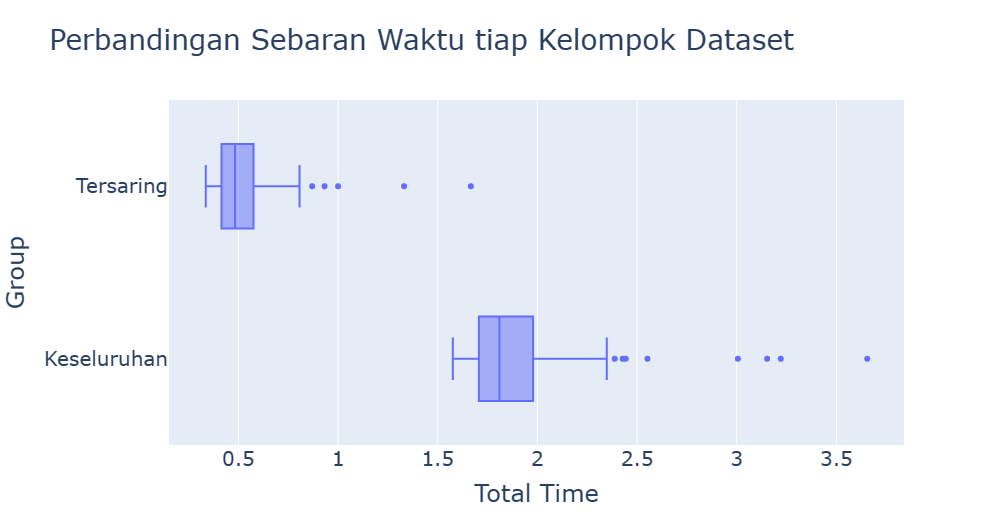
\includegraphics[width=\textwidth]{perbandingan_dataset400.png}
	\caption{Perbandingan sebaran waktu Dataset 400.}
	\label{fig:perbandingan_dataset400}
\end{figure}
Dari gambar tersebut terlihat bahwa ada perbedaan sebaran nilai yang besar antara dataset yang telah disaring dan keseluruhan. Dataset yang telah disaring memiliki total waktu yang tersebar pada nilai-nilai yang lebih kecil dibandingkan dengan dataset secara keseluruhan. Untuk perbandingan total waktu serta akurasi dari dataset keseluruhan dan yang telah disaring dapat dilihat pada tabel berikut:

\begin{table}[H]
	\centering
	\begin{tabular}{|cc|cc|}
		\hline
		\multicolumn{2}{|c|}{\textbf{Keseluruhan}}                        & \multicolumn{2}{c|}{\textbf{Disaring}}                           \\ \hline
		\multicolumn{1}{|l|}{Total Waktu (detik)} & Akurasi (\%) & \multicolumn{1}{l|}{Total Waktu (detik)} & Akurasi (\%) \\ \hline
		\multicolumn{1}{|l|}{82.15}               & 98           & \multicolumn{1}{l|}{31.79}               & 96           \\ \hline
	\end{tabular}
\end{table}

Dari tabel di atas terlihat bahwa penyaringan pada fitur lokal meningkatkan waktu pemrosesan yang dapat dilihat dari penurunan total waktu yang signifikan (61.3\%). Penurunan waktu tersebut dikarenakan jumlah fitur lokal yang diproses lebih sedikit. Walaupun begitu penurunan akurasi dari saat menggunakan keseluruhan data ke penggunaan data yang disaring tidak cukup signifikan. Akurasi hanya menurun sebanyak 2\%. 

Hasil tersebut menunjukkan adanya peningkatan performa BSIS dari segi waktu jika menggunakan fitur lokal yang sudah disaring terlebih dahulu. Walaupun akurasi juga menurun tetapi penurunan akurasi tidak cukup signifikan jika dibandingkan dengan peningkatan kecepatan.

\subsubsection{Dataset 600}
Dataset 600 memiliki total fitur lokal yang dihasilkan dari seluruh gambar sebanyak 49976 fitur lokal. Setelah dilakukan \textit{clustering} menghitung nilai keunikan dan konsistensi didapat hasil sebaran nilai keunikan dan konsistensi seperti pada Gambar~\ref{fig:half_600_uniqueness} dan Gambar~\ref{fig:half_600_consistency}.
\begin{figure}[H]
	\centering
	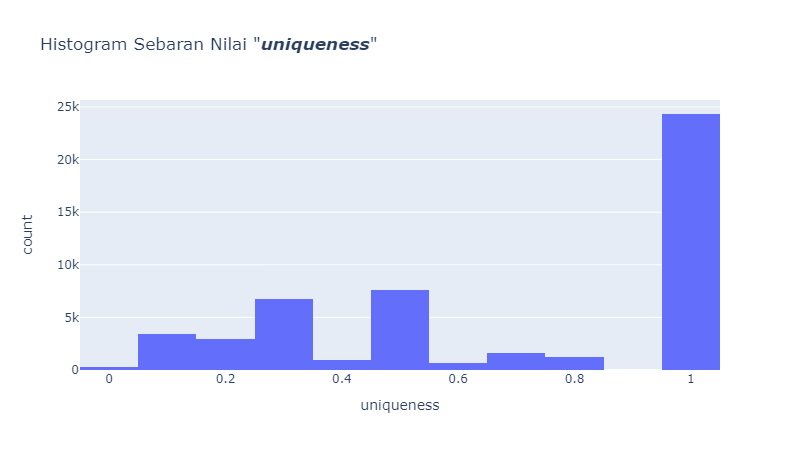
\includegraphics[width=\textwidth]{half_600_uniqueness.png}
	\caption{Sebaran nilai keunikan (\texttt{uniqueness}) untuk Dataset 600.}
	\label{fig:half_600_uniqueness}
\end{figure}
\begin{figure}[H]
	\centering
	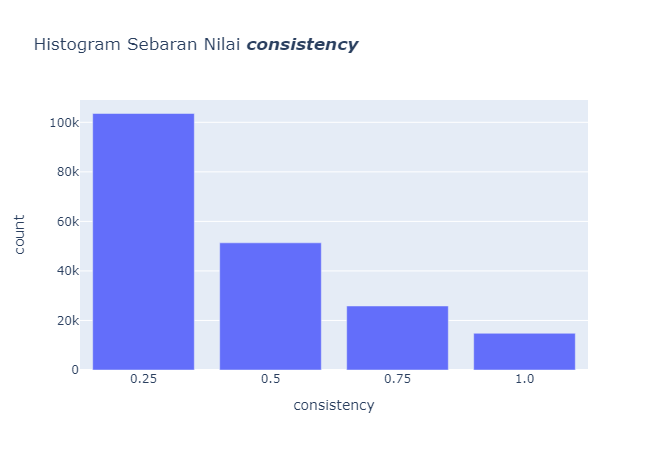
\includegraphics[width=\textwidth]{half_600_consistency.png}
	\caption{Sebaran nilai keunikan (\texttt{consistency}) untuk Dataset 600.}
	\label{fig:half_600_consistency}
\end{figure}
Berdasarkan sebaran data tersebut ditentukan batas untuk nilai keunikan (\texttt{uniqueness}) adalah $> 0.99$ dan untuk konsistensi (\texttt{consistency}) adalah $> 0.49$. Setelah data disaring menggunakan batas-batas tersebut didapatkan total sebanyak 13853 fitur lokal. Data keseluruhan dan data yang telah disaring tersebut lalu digunakan untuk pengenalan gambar \textit{test}. 
Hasil pengenalan gambar \textit{test} pada dataset keseluruhan dapat dilihat potongannya pada Tabel~\ref{tab:result_full_600}.
\begin{table}[H]
	\centering
	\begin{tabular}{|c|c|c|c|c|c|c|} 
		\hline
		& \textbf{q\_name} & \textbf{t\_name} & \textbf{kdtree\_time} & \textbf{total\_time} & \textbf{total\_weight} & \textbf{is\_true}  \\ 
		\hline
		0   & 001-test0.jpg    & 001-iPhone.jpg   & 1.245                 & 1.354                & 151.124                & 1                  \\ 
		\hline
		1   & 001-test1.jpg    & 001-iPhone.jpg   & 1.156                 & 1.248                & 132.160                & 1                  \\ 
		\hline
		2   & 002-test0.jpg    & 002-iPhone.jpg   & 1.051                 & 1.106                & 110.707                & 1                  \\ 
		\hline
		3   & 002-test1.jpg    & 002-Droid.jpg    & 1.050                 & 1.095                & 69.215                 & 1                  \\ 
		\hline
		4   & 003-test0.jpg    & 003-iPhone.jpg   & 1.082                 & 1.158                & 154.965                & 1                  \\ 
		\hline
		5   & 003-test1.jpg    & 003-Droid.jpg    & 1.090                 & 1.181                & 117.895                & 1                  \\ 
		\hline
		6   & 004-test0.jpg    & 004-iPhone.jpg   & 1.037                 & 1.077                & 248.097                & 1                  \\ 
		\hline
		7   & 004-test1.jpg    & 004-iPhone.jpg   & 1.126                 & 1.259                & 394.791                & 1                  \\ 
		\hline
		8   & 005-test0.jpg    & 005-Droid.jpg    & 0.917                 & 1.040                & 775.478                & 1                  \\ 
		\hline
		9   & 005-test1.jpg    & 005-Droid.jpg    & 0.743                 & 0.873                & 578.210                & 1                  \\ 
		\hline
		... & ...              & ...              & ...                   & ...                  & ...                    & ...                \\ 
		\hline
		90  & 046-test0.jpg    & 046-Droid.jpg    & 0.682                 & 0.714                & 98.835                 & 1                  \\ 
		\hline
		91  & 046-test1.jpg    & 046-Droid.jpg    & 0.699                 & 0.751                & 146.754                & 1                  \\ 
		\hline
		92  & 047-test0.jpg    & 047-iPhone.jpg   & 0.679                 & 0.730                & 303.266                & 1                  \\ 
		\hline
		93  & 047-test1.jpg    & 047-iPhone.jpg   & 0.668                 & 0.682                & 18.561                 & 1                  \\ 
		\hline
		94  & 048-test0.jpg    & 048-iPhone.jpg   & 0.652                 & 0.676                & 270.232                & 1                  \\ 
		\hline
		95  & 048-test1.jpg    & 048-iPhone.jpg   & 0.650                 & 0.667                & 166.423                & 1                  \\ 
		\hline
		96  & 049-test0.jpg    & 049-iPhone.jpg   & 0.710                 & 0.789                & 297.539                & 1                  \\ 
		\hline
		97  & 049-test1.jpg    & 049-iPhone.jpg   & 0.696                 & 0.765                & 311.168                & 1                  \\ 
		\hline
		98  & 050-test0.jpg    & 050-Canon.jpg    & 0.871                 & 1.037                & 103.319                & 1                  \\ 
		\hline
		99  & 050-test1.jpg    & 004-iPhone.jpg   & 0.802                 & 0.915                & 43.560                 & 0                  \\
		\hline
	\end{tabular}	
	\caption{Beberapa contoh hasil BSIS pada keseluruhan Dataset 600.}
	\label{tab:result_full_600}
\end{table}

Sedangkan untuk hasil pada data yang telah disaring beberapa potongannya adalah seperti dapat dilihat pada Tabel~\ref{tab:result_filtered_600}
\begin{table}[H]
	\centering
	\begin{tabular}{|c|c|c|c|c|c|c|} 
		\hline
		& \textbf{q\_name} & \textbf{t\_name} & \textbf{kdtree\_time} & \textbf{total\_time} & \textbf{total\_weight} & \textbf{is\_true}  \\ 
		\hline
		0   & 001-test0.jpg    & 001-iPhone.jpg   & 0.406                 & 0.519                & 61.144                 & 1                  \\ 
		\hline
		1   & 001-test1.jpg    & 001-Droid.jpg    & 0.383                 & 0.469                & 58.070                 & 1                  \\ 
		\hline
		2   & 002-test0.jpg    & 002-iPhone.jpg   & 0.333                 & 0.375                & 87.264                 & 1                  \\ 
		\hline
		3   & 002-test1.jpg    & 002-iPhone.jpg   & 0.335                 & 0.373                & 37.118                 & 1                  \\ 
		\hline
		4   & 003-test0.jpg    & 003-iPhone.jpg   & 0.353                 & 0.421                & 109.130                & 1                  \\ 
		\hline
		5   & 003-test1.jpg    & 003-iPhone.jpg   & 0.340                 & 0.419                & 79.736                 & 1                  \\ 
		\hline
		6   & 004-test0.jpg    & NaN              & 0.292                 & 0.312                & 0.000                  & 0                  \\ 
		\hline
		7   & 004-test1.jpg    & 047-iPhone.jpg   & 0.373                 & 0.475                & 41.536                 & 0                  \\ 
		\hline
		8   & 005-test0.jpg    & 005-Droid.jpg    & 0.380                 & 0.534                & 263.913                & 1                  \\ 
		\hline
		9   & 005-test1.jpg    & 005-Droid.jpg    & 0.398                 & 0.574                & 378.274                & 1                  \\ 
		\hline
		... & ...              & ...              & ...                   & ...                  & ...                    & ...                \\ 
		\hline
		90  & 046-test0.jpg    & 046-Droid.jpg    & 0.199                 & 0.227                & 29.213                 & 1                  \\ 
		\hline
		91  & 046-test1.jpg    & 046-Droid.jpg    & 0.213                 & 0.261                & 82.782                 & 1                  \\ 
		\hline
		92  & 047-test0.jpg    & 047-iPhone.jpg   & 0.203                 & 0.239                & 66.674                 & 1                  \\ 
		\hline
		93  & 047-test1.jpg    & NaN              & 0.191                 & 0.203                & 0.000                  & 0                  \\ 
		\hline
		94  & 048-test0.jpg    & 048-iPhone.jpg   & 0.178                 & 0.199                & 193.285                & 1                  \\ 
		\hline
		95  & 048-test1.jpg    & 048-iPhone.jpg   & 0.179                 & 0.191                & 143.975                & 1                  \\ 
		\hline
		96  & 049-test0.jpg    & 049-iPhone.jpg   & 0.231                 & 0.313                & 276.651                & 1                  \\ 
		\hline
		97  & 049-test1.jpg    & 049-iPhone.jpg   & 0.214                 & 0.276                & 243.250                & 1                  \\ 
		\hline
		98  & 050-test0.jpg    & 050-Canon.jpg    & 0.370                 & 0.536                & 43.878                 & 1                  \\ 
		\hline
		99  & 050-test1.jpg    & 027-Droid.jpg    & 0.303                 & 0.420                & 20.752                 & 0                  \\
		\hline
	\end{tabular}
	\caption{Beberapa contoh hasil BSIS pada Dataset 600 yang telah disaring berdasarkan \texttt{uniqueness} dan \texttt{consistency}.}
	\label{tab:result_filtered_600}
\end{table}

Perbedaan sebaran waktu yang digunakan untuk tiap gambar pada saat digunakan data secara keseluruhan dan yang telah disaring dapat dilihat pada Gambar~\ref{fig:perbandingan_dataset600}.
\begin{figure}[H]
	\centering
	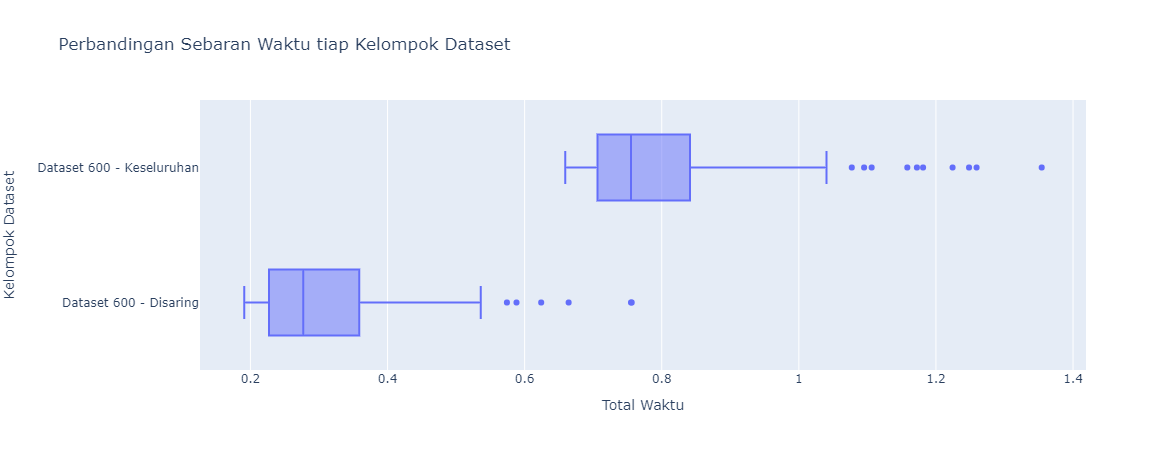
\includegraphics[width=\textwidth]{perbandingan_dataset600.png}
	\caption{Perbandingan sebaran waktu Dataset 600.}
	\label{fig:perbandingan_dataset600}
\end{figure}
Dari gambar tersebut terlihat bahwa ada perbedaan sebaran nilai yang besar antara dataset yang telah disaring dan keseluruhan. Dataset yang telah disaring memiliki total waktu yang tersebar pada nilai-nilai yang lebih kecil dibandingkan dengan dataset secara keseluruhan. Untuk perbandingan total waktu serta akurasi dari dataset keseluruhan dan yang telah disaring dapat dilihat pada tabel berikut:

\begin{table}[H]
	\centering
	\begin{tabular}{|cc|cc|}
		\hline
		\multicolumn{2}{|c|}{\textbf{Keseluruhan}}                        & \multicolumn{2}{c|}{\textbf{Disaring}}                           \\ \hline
		\multicolumn{1}{|l|}{Total Waktu (detik)} & Akurasi (\%) & \multicolumn{1}{l|}{Total Waktu (detik)} & Akurasi (\%) \\ \hline
		\multicolumn{1}{|l|}{80.96}               & 96           & \multicolumn{1}{l|}{31.41}               & 89           \\ \hline
	\end{tabular}
\end{table}

Dari tabel di atas terlihat bahwa penyaringan pada fitur lokal meningkatkan waktu pemrosesan yang dapat dilihat dari penurunan total waktu yang signifikan (61.2\%). Penurunan waktu tersebut dikarenakan jumlah fitur lokal yang diproses lebih sedikit. Tetapi penurunan akurasi dari saat menggunakan keseluruhan data ke penggunaan data yang disaring juga cukup signifikan. Akurasi menurun sebanyak 7\%

Hasil tersebut menunjukkan adanya peningkatan performa BSIS dari segi waktu jika menggunakan fitur lokal yang sudah disaring terlebih dahulu. Walaupun akurasi juga menurun tetapi juga terjadi penurunan yang signifikan pada nilai akurasi.

\subsubsection{Perbandingan Dataset 400 dan Dataset 600}
Percobaan yang dilakukan dengan menggunakan Dataset 400 dan Dataset 600 memiliki perbedaan yang cukup terlihat dari sisi akurasi yang dihasilkan. Perbandingan tersebut dapat dilihat pada tabel berikut:
\begin{table}[H]
	\centering
	\begin{tabular}{|c|c|c|c|c|} 
		\hline
		& \multicolumn{2}{c|}{\textbf{Keseluruhan}}   & \multicolumn{2}{c|}{\textbf{Disaring}}       \\ 
		\hline
		& Total Waktu (detik) & Akurasi (\%) & Total Waktu (detik) & Akurasi (\%)  \\ 
		\hline
		\textbf{Dataset 400} & 82.15               & 98           & 31.78               & 96            \\ 
		\hline
		\textbf{Dataset 600} & 80.96               & 96           & 31.41               & 89            \\
		\hline
	\end{tabular}
\end{table}

Tabel di atas menunjukkan bahwa penggunaan Dataset 400 memberikan hasil yang lebih baik dari Dataset 600. Terutama pada saat penggunaan dataset yang disaring, akurasi dari Dataset 400 mencapai 96\% sedangkan untuk Dataset 600 hanya 89\% dengan perbedaan waktu yang sangat sedikit.

Dataset 400 memiliki hasil yang lebih baik kemungkinan dikarenakan ukuran gambar pada Dataset 400 lebih mendekati ukuran dari gambar-gambar di data \textit{test}. Karena ukuran yang mirip tersebut maka fitur lokal yang dihasilkan memiliki ciri yang lebih mirip.

\section{Analisis Pengaruh Parameter Agglomerative Clustering terhadap Sebaran Nilai Keunikan dan Konsistensi}
\label{sec:analisis_parameter_clustering}
Nilai keunikan dan konsistensi dari hasil \textit{clustering} pada tahap sebelumnya tidak tersebar secara merata. Terutama pada nilai keunikan mayoritas data memiliki nilai keunikan 1. Karena sebaran yang terpusat pada nilai 1 ini penyaringan data dengan mengatur nilai keunikan tidak memberikan perbedaan berarti. 

Analisis yang dilakukan pada \ref{sec:analisis_bsis} menggunakan nilai keunikan dan konsistensi yang didapat dengan menggunakan metode \textit{Agglomerative Clustering} sesuai dengan yang dilakukan pada \ref{sec:analisis_sifat}. Metode \textit{Agglomerative Clustering} yang dilakukan pada \ref{sec:analisis_sifat} membagi \textit{cluster} berdasarkan pada parameter \texttt{distance\_threshold} yang di mana pada analisis tersebut didapat dari setengah nilai rata-rata jarak antar data sampel. Pada analisis ini akan diuji apakah dengan mengubah nilai \texttt{distance\_threshold} dapat mengubah sebaran nilai keunikan dan konsistensi sehingga jumlah fitur lokal yang digunakan dapat lebih mudah diubah dengan mengatur nilai batas konsistensi dan keunikan.

Dataset yang digunakan pada analisis ini sama seperti analisis sebelumnya yaitu menggunakan dataset Book Covers tetapi hanya menggunakan satu ukuran yaitu Dataset 400. Dataset 400 digunakan pada penelitian ini karena dari hasil sebelumnya didapat bahwa Dataset ini memberikan hasil yang terbaik.

\subsection{Ide Analisis dan Tahapan}
Analisis dilakukan dengan mengubah nilai parameter \texttt{distance\_threshold} di \textit{Agglomerative Clustering} menjadi nilai rata-rata jarak antar data sampel. Nilai \texttt{distance\_threshold} yang lebih tinggi akan membuat lebih mudah untuk data menjadi tergabung dalam satu \textit{cluster}. \textit{Cluster-cluster} yang dihasilkan akan lebih sedikit dan dengan jumlah data di tiap \textit{cluster}-nya lebih banyak.

Analisis akan dilakukan pada bagaimana sebaran nilai keunikan dan konsistensi. Bagaimana menentukan batas dari sebaran nilai tersebut dan apakah fitur lokal yang didapat dari hasil penyaringan akan menghasilkan nilai akurasi yang berbeda jika digunakan sebagai dataset dalam identifikasi dengan BSIS.

Tahapan yang dilakukan sama dengan tahapan pada \ref{sec:analisis_sifat} untuk menghitung nilai keunikan dan konsistensi. Setelah didapatkan nilai tersebut dilakukan identifikasi dengan BSIS dengan tahapan yang sama dengan tahapan pada \ref{sec:analisis_bsis}.

\subsection{Hasil Analisis}
Setelah dilakukan \textit{clustering} untuk menghitung nilai keunikan dan konsistensi didapat sebaran nilai seperti pada gambar-gambar berikut ini. Gambar~\ref{fig:half_400_uniqueness_1} menunjukkan sebaran nilai keunikan dan Gambar~\ref{fig:half_400_consistency_1} menunjukkan sebaran nilai konsistensi.
\begin{figure}[H]
	\centering
	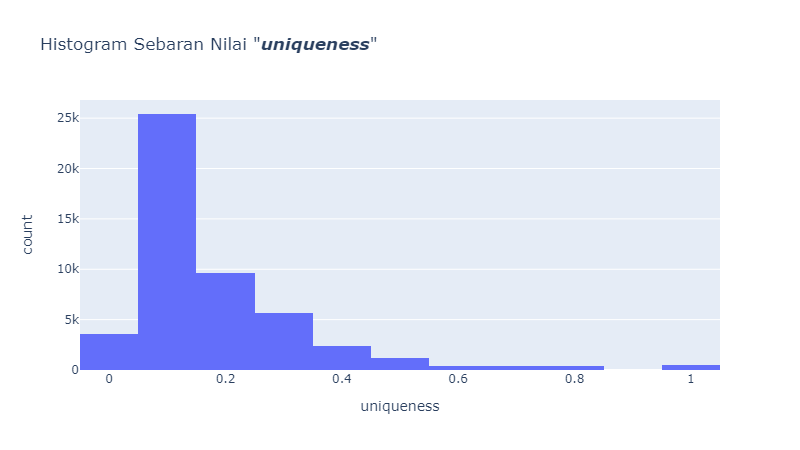
\includegraphics[width=\textwidth]{half_400_uniqueness_1.png}
	\caption{Sebaran nilai keunikan (\texttt{uniqueness}) untuk Dataset 400 saat menggunakan parameter \textit{Agglomerative Clustering} yang berbeda.}
	\label{fig:half_400_uniqueness_1}
\end{figure}
\begin{figure}[H]
	\centering
	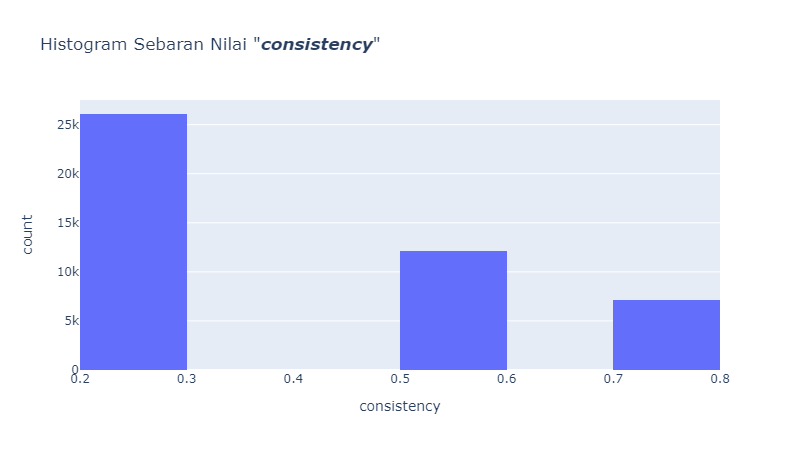
\includegraphics[width=\textwidth]{half_400_consistency_1.png}
	\caption{Sebaran nilai keunikan (\texttt{consistency}) untuk Dataset 400 saat menggunakan parameter \textit{Agglomerative Clustering} yang berbeda.}
	\label{fig:half_400_consistency_1}
\end{figure}
Sebaran nilai konsistensi seperti yang terlihat pada Gambar~\ref{fig:half_400_consistency_1} memiliki pola yang sama seperti sebaran pada saat menggunakan setengah rata-rata jarak sebagai \texttt{distance\_threshold}. Sedangkan untuk nilai keunikan sebaran datanya memiliki pola yang berbeda dari analisis sebelumnya saat menggunakan setengah rata-rata jarak. Pada analisis sebelumnya tingkat fitur lokal dengan tingkat keunikan 1 mendominasi dataset, tetapi pada analisis ini tingkat keunikan fitur lokal justru mayoritas berada di kisaran yang rendah (0.05 - 0.2). 

Pada analisis sebelumya karena mayoritas nilai keunikan ada pada nilai 1 maka perubahan pada batas bawah nilai keunikan saat melakukan penyaringan terhadap fitur lokal tidak akan berdampak pada hasil fitur lokal yang didapat. Tetapi pada penelitian kali ini karena sebaran nilai keunikannya lebih merata dan mayoritas tersebar pada rentang nilai-nilai kecil maka perubahan nilai batas bawah untuk menyaring fitur lokal akan berpengaruh pada jumlah fitur lokal yang didapat.

\section{Analisis Pengaruh Batas Nilai Keunikan yang Digunakan terhadap Jumlah Fitur Lokal yang Didapat dan Tingkat Akurasi BSIS}
\label{sec:analisis_batas_keunikan}
Pada analisis di \ref{sec:analisis_parameter_clustering} didapati bahwa dengan menggunakan nilai parameter \texttt{distance\_threshold} di \textit{Agglomerative Clustering} yang lebih besar menyebabkan \textit{cluster-cluster} yang dihasilkan memiliki ciri berbeda. \textit{Cluster} dengan ciri berbeda tersebut memengaruhi nilai keunikan dari fitur lokal. Nilai keunikan fitur lokal jadi tersebar secara lebih merata dan terpusat pada nilai pada rentang yang kecil.

Nilai fitur lokal yang lebih tersebar memungkinkan untuk dilakukan penyaringan dengan batas bawah yang berbeda dan didapatkan hasil yang berbeda. Pada bagian ini akan dilakukan analisis untuk mengetahui bagaimana pengaruh penentuan nilai batas bawah terhadap jumlah fitur lokal yang tersaring dan bagaimana pengaruhnya terhadap tingkat akurasi saat data tersebut digunakan untuk identifikasi dengan BSIS.

\subsection{Ide Analisis dan Tahapan}
Penelitian akan dilakukan dengan melakukan tahapan yang sama seperti pada penelitian di \ref{sec:analisis_bsis}. Tetapi pada penelitian ini yang dibandingkan adalah nilai akurasi dan total waktu dari beberapa hasil penyaringan dataset dengan menggunakan batas nilai keunikan yang berbeda. Untuk setiap batas nilai keunikan yang digunakan akan dihitung berapa fitur lokal yang tersisa dan nilai akurasi serta total waktu pemrosesan.

Pada penelitian ini akan digunakan 3 batas nilai keunikan yang berbeda yaitu: 0.2, 0.4, dan 0.6 sedangkan untuk batas nilai konsistensi hanya akan digunakan 0.49 untuk setiap batas nilai keunikan. Dataset untuk data \textit{train} yang digunakan adalah dataset yang sama dengan Dataset 400 pada \ref{sec:analisis_bsis}. Sedangkan untuk data \textit{test} digunakan data yang sama dengan dataset \textit{test} pada \ref{sec:analisis_bsis}.

Tahapan analisis yang dilakukan adalah sebagai berikut:
\begin{enumerate}
	\item \textit{Load} Gambar \\
	\textit{Load} semua gambar \textit{test} yang digunakan.
	\item \textit{Load} Dataset \\
	\textit{Load} dataset yang digunakan (Dataset 400) dan saring data tersebut berdasarkan batas nilai keunikan serta konsistensi yang digunakan pada tahap ini. Dihitung juga jumlah data yang tersaring.
	\item Identifikasi dengan BSIS \\
	Lakukan identifikasi BSIS pada gambar \textit{test} dengan menggunakan dataset yang telah disaring.
	\item Penghitungan Akurasi Serta \\
	Menghitung total waktu yang digunakan untuk menyelesaikan seluruh gambar dan berapa gambar yang mendapat hasil benar.
\end{enumerate}
Langkah-langkah tahapan tersebut dilakukan untuk setiap batas keunikan yang digunakan (0.2, 0.4, dan 0.6). Hasilnya lalu disimpan dan dibandingkan.

\subsection{Hasil Analisis}
Setelah dilakukan seluruh tahapan di atas didapatkan hasil sebagai seperti pada Tabel~\ref{tab:nilai_keunikan}. Ditulis juga total waktu dan akurasi 
\begin{table}[H]
	\centering
	\begin{tabular}{|c|c|c|c|}
		\hline
		Batas Nilai Keunikan & Jumlah Fitur Lokal & Total Waktu (detik) & Akurasi (\%) \\
		\hline
		0.2 & 11627 & 30.31 & 95 \\
		\hline
		0.4 & 3484 & 17.12 & 63 \\
		\hline
		0.6 & 1232 & 13.20 & 37 \\
		\hline
	\end{tabular}
	\caption{Perbedaan hasil dari setiap penggunaan batas nilai keunikan yang berbeda.}
	\label{tab:nilai_keunikan}
\end{table}
Dari tabel tersebut terlihat bahwa penggunaan nilai batas yang tinggi memberikan jumlah fitur lokal yang semakin sedikit. Fitur lokal yang sedikit membuat pemrosesan waktu menjadi lebih cepat tetapi juga berdampak pada akurasi. Penggunaan jumlah fitur lokal yang terlalu sedikit menyebabkan nilai akurasi menjadi sangat rendah seperti ditunjukkan pada penggunaan nilai batas 0.4 dan 0.6.

Berdasarkan data Tabel~\ref{tab:nilai_keunikan} dapat disimpulkan bahwa perlu untuk memilih batas nilai yang tepat untuk mendapatkan hasil deteksi yang cepat dan dengan akurasi yang tinggi. Seperti penggunaan nilai keunikan 0.2, fitur lokal yang didapat cukup berbeda jumlahnya dengan jika digunakan semua fitur lokal dan waktu pemrosesan juga lebih singkat secara signifikan (penggunaan semua fitur lokal memiliki waktu pemrosesan selama 82.15), tetapi nilai akurasinya masih termasuk tinggi.
